%! TeX program = xelatex

\documentclass[xetex,aspectratio=169,xcolor,professionalfonts,hyperref]{beamer}
\usepackage[
    style=authoryear,
    backend=biber,
    natbib,
    uniquename=false,
    maxcitenames=2,
    maxbibnames=20,
    sorting=nty]{biblatex}
\addbibresource{refs.bib}
\renewcommand*{\bibfont}{\scriptsize}
\usepackage{anyfontsize}
\usepackage{tabularx}
\usepackage{changepage}
\usetheme{dark18}
\usepackage{stmaryrd}
\usepackage{nicefrac}
\usepackage{graphicx}
\usepackage{stackrel}
\usepackage{booktabs}
\usepackage{xspace}
\usepackage{tikz-dependency}
\usepackage{tkz-graph}
\usepackage{pgfplots}
\usepgfplotslibrary{groupplots}
% emojis!
\makeatletter
\newcommand*\fsize{\dimexpr\f@size pt\relax}
\makeatother
\newcommand*\emoji[2][1]{\includegraphics[width=#1\fsize]{emoji/#2}}
%
%% Generic TiKZ utils!
\usetikzlibrary{calc,backgrounds,arrows,arrows.meta}
\usetikzlibrary{decorations.pathreplacing}
\usetikzlibrary{tikzmark,positioning,patterns}
\usetikzlibrary{bending}
\usetikzlibrary{overlay-beamer-styles}
\pgfdeclarelayer{background}
\pgfdeclarelayer{foreground}
\pgfsetlayers{background,main,foreground}
%
\tikzset{
    visible on/.style={alt={#1{}{invisible}}},
    invisible/.style={opacity=0},
    alt/.code args={<#1>#2#3}{%
      \alt<#1>{\pgfkeysalso{#2}}{\pgfkeysalso{#3}} % \pgfkeysalso doesn't change the path
    },
  }

%% particular stuff?
\newcommand*{\ticksize}{2pt}
\tikzset{axisline/.style={thick,myfg!50!mybg,text=myfg,font=\small}}
\tikzset{axislabel/.style={font=\small}}
\tikzset{point/.style={thick,tMidnight}}


% semantic color definitions
\colorlet{colorArgmax}{tTarmac}
\colorlet{colorSoftmax}{tVividBlue}
\colorlet{colorSparsemax}{tYellow!50}
\colorlet{colorFusedmax}{tPeony!80!mybg}
\colorlet{colorEntmax}{tPeony}


\tikzset{
    tinyarrowl/.style={-{Straight Barb[bend]},thick,bend left=75,tPeony},
    tinyarrowr/.style={-{Straight Barb[bend]},thick,bend right=75,tPeony}}
\newcommand{\miniparse}[1]{%
{\footnotesize%
\begin{tikzpicture}[
    node distance=14pt,
    every node/.style={inner sep=0,outer sep=1pt},
    ]
\node[tPeony] (a) at (0, 0) {\textbullet};
\node[tPeony,right of=a] (b) {\textbullet};
\node[tPeony,right of=b] (c) {\textbullet};
\foreach \i/\j/\r/\o in {#1}{
\path (\i.north) edge[tinyarrow\r,opacity=\o] (\j.north);
}\end{tikzpicture}}}

% Tikz pic: draw a cog
\tikzset{cog/.pic={code={
    \draw[myfg,thick,fill=tTarmac!90]
  (0:2)
  \foreach \i [evaluate=\i as \n using {(\i-1)*360/18}] in {1,...,18}{%
    arc (\n:\n+10:2) {[rounded corners=1.5pt] -- (\n+10+2:2.4)
    arc (\n+10+2:\n+360/18-2:2.4)} --  (\n+360/18:2)
  };
  \draw[myfg,thick,fill=mybg] (0,0) circle[radius=.5];
}}}
%
%
% Tikz: draw an envelope
\newsavebox\envelope
\savebox{\envelope}{

\newlength\mylen
\setlength\mylen{2cm}
\begin{tikzpicture}[scale=.65]

\coordinate (A) at (0,0);
\coordinate (B) at (1.41\mylen,-\mylen);
\clip
  ([xshift=-0.5\pgflinewidth,yshift=0.5\pgflinewidth]A) --
  ([xshift=0.5\pgflinewidth,yshift=0.5\pgflinewidth]A-|B) --
  ([xshift=0.5\pgflinewidth,yshift=-0.5\pgflinewidth]B) --
  ([xshift=-0.5\pgflinewidth,yshift=-0.5\pgflinewidth]B-|A) --
  ([xshift=-0.5\pgflinewidth,yshift=0.5\pgflinewidth]A);
\draw[mybg,fill=tTarmac,line cap=rect]
  (A) -- (A-|B) -- (B) -- (B-|A) -- (A);
\draw[mybg]
  (B-|A) -- (0.705\mylen,-.3\mylen) -- (B);
\draw[mybg,fill=tTarmac!90,rounded corners=15pt]
  (A) -- (0.705\mylen,-0.6\mylen) -- (A-|B);
\node[anchor=north]
  at ($ (A)!0.5!(B|-A) $ ) {\parbox{\mylen}{}};
\draw[mybg] (A) -- (B|-A);
\end{tikzpicture}
}
%
% output
\newsavebox\sentoutput
\savebox{\sentoutput}{%
    \begin{tikzpicture}[scale=.75,text=myfg]
 \draw[rounded corners,tTarmac!60,very thick] (-.5, -.5) rectangle (.5, 2.5) {};

 \node[label={[label distance=.25cm]0:positive}] (pos) at (0, 2) {};
 \node[label={[label distance=.25cm]0:neutral}] (neu) at (0, 1) {};
 \node[label={[label distance=.25cm]0:negative}] (neg) at (0, 0) {};

 \draw[fill=tNavy!80!myfg] (pos) circle[radius=9pt];
 \draw[fill=tNavy!20!myfg] (neu) circle[radius=9pt];
 \draw[fill=tNavy!20!myfg] (neg) circle[radius=9pt];
 \end{tikzpicture}
 }
%
% cartoon structure
\newcommand{\cartoon}[2][1]{%
\begin{tikzpicture}%
\node[draw=none, minimum size=#1*1cm, regular polygon, regular polygon sides=5] (p) {};
%
\foreach \i/\j in {#2}%
{
    \draw[tPeony, ultra thick] (p.corner \i) -- (p.corner \j);
}
%
\foreach \i in {1, ..., 5}%
{
    \draw[myfg,fill=mybg,very thick] (p.corner \i) circle[radius=#1*5pt];
}
\end{tikzpicture}}
\newcommand{\cartoonDense}[1][1]{%
\begin{tikzpicture}%
\node[draw=none, minimum size=#1*1cm, regular polygon, regular polygon sides=5] (p) {};
%
\draw[tPeony, ultra thick, opacity=.8] (p.corner 1) -- (p.corner 2);
\draw[tPeony, ultra thick, opacity=.5] (p.corner 1) -- (p.corner 3);
\draw[tPeony, ultra thick, opacity=.7] (p.corner 1) -- (p.corner 4);
\draw[tPeony, ultra thick, opacity=.4] (p.corner 1) -- (p.corner 5);
\draw[tPeony, ultra thick, opacity=.6] (p.corner 2) -- (p.corner 3);
\draw[tPeony, ultra thick, opacity=.3] (p.corner 2) -- (p.corner 4);
\draw[tPeony, ultra thick, opacity=.9] (p.corner 2) -- (p.corner 5);
\draw[tPeony, ultra thick, opacity=.2] (p.corner 3) -- (p.corner 4);
\draw[tPeony, ultra thick, opacity=.6] (p.corner 3) -- (p.corner 5);
\draw[tPeony, ultra thick, opacity=.4] (p.corner 4) -- (p.corner 5);
%
\foreach \i in {1, ..., 5}%
{
    \draw[myfg,fill=mybg,very thick] (p.corner \i) circle[radius=#1*5pt];
}
\end{tikzpicture}}
\newcommand{\cartoonSparse}[1][1]{%
\begin{tikzpicture}%
\node[draw=none, minimum size=#1*1cm, regular polygon, regular polygon sides=5] (p) {};
%
\draw[tPeony, ultra thick, opacity=1] (p.corner 1) -- (p.corner 4);
\draw[tPeony, ultra thick, opacity=.5] (p.corner 2) -- (p.corner 5);
\draw[tPeony, ultra thick, opacity=.5] (p.corner 1) -- (p.corner 5);
%
\foreach \i in {1, ..., 5}%
{
    \draw[myfg,fill=mybg,very thick] (p.corner \i) circle[radius=#1*5pt];
}
\end{tikzpicture}}
%
\newcommand{\setupsimplexbary}[1][3.3]{%
\coordinate (L1) at (0:0);
\coordinate (L2) at (0:#1);
\coordinate (L3) at (60:#1);

\node[label=east:{\small$\triangle$}] at (L2) {};

\fill[tYellow,opacity=.15]  (L1) -- (L2) -- (L3) -- cycle;
\draw[very thick,tYellow] (L1) -- (L2) -- (L3) -- cycle;

\draw[tYellow,fill] (L1) circle[radius=3pt];
\draw[tYellow,fill] (L2) circle[radius=3pt];
\draw[tYellow,fill] (L3) circle[radius=3pt];
}

\newcommand{\drawcs}{%
\node[anchor=south] at (0, \vecheight*4) {$c_1$};
\node[anchor=south] at (0, \vecheight*3) {$c_2$};
\node[anchor=south] at (0, \vecheight*1.5) {$\cdots$};
\node[anchor=south] at (0, \vecheight*0) {$c_N$};}

\newcommand{\drawscores}{%
\node[anchor=south] at (-1-.5*\vecwidth, \vecheight*5+.1) {$\s$};
\draw[elem,fill=vecfg!60!vecbg] (-1-\vecwidth, \vecheight*4) rectangle (-1, \vecheight*5);
\draw[elem,fill=vecfg!85!vecbg] (-1-\vecwidth, \vecheight*3) rectangle (-1, \vecheight*4);
\draw[elem,fill=vecfg!60!vecbg] (-1-\vecwidth, \vecheight*2) rectangle (-1, \vecheight*3);
\draw[elem,fill=vecfg!75!vecbg] (-1-\vecwidth, \vecheight*1) rectangle (-1, \vecheight*2);
\draw[elem,fill=vecfg!50!vecbg] (-1-\vecwidth, \vecheight*0) rectangle (-1, \vecheight*1);
}

\newcommand{\drawargmax}{%
\node[anchor=south] at (1+.5*\vecwidth, \vecheight*5+.1) {$\p$};
\draw[elem,fill=vecfg! 0!vecbg]  (1, \vecheight*4) rectangle (1+\vecwidth, \vecheight*5);
\draw[elem,fill=vecfg!70!vecbg]  (1, \vecheight*3) rectangle (1+\vecwidth, \vecheight*4);
\draw[elem,fill=vecfg! 0!vecbg]  (1, \vecheight*2) rectangle (1+\vecwidth, \vecheight*3);
\draw[elem,fill=vecfg! 0!vecbg]  (1, \vecheight*1) rectangle (1+\vecwidth, \vecheight*2);
\draw[elem,fill=vecfg! 0!vecbg]  (1, \vecheight*0) rectangle (1+\vecwidth, \vecheight*1);
}
\newcommand{\drawsoftmax}{%
\node[anchor=south] at (1+.5*\vecwidth, \vecheight*5+.1) {$\p$};
\draw[elem,fill=vecfg!30!vecbg]  (1, \vecheight*4) rectangle (1+\vecwidth, \vecheight*5);
\draw[elem,fill=vecfg!50!vecbg]  (1, \vecheight*3) rectangle (1+\vecwidth, \vecheight*4);
\draw[elem,fill=vecfg!35!vecbg]  (1, \vecheight*2) rectangle (1+\vecwidth, \vecheight*3);
\draw[elem,fill=vecfg!25!vecbg]  (1, \vecheight*1) rectangle (1+\vecwidth, \vecheight*2);
\draw[elem,fill=vecfg!15!vecbg]  (1, \vecheight*0) rectangle (1+\vecwidth, \vecheight*1);
}


% math and notation
\newcommand*\bs[1]{\boldsymbol{#1}}
\newcommand\defeq{{\,\raisebox{1pt}{$:$}=}\,}
\newcommand\p{\bs{p}}
\newcommand\xx{z}
\newcommand\x{\bs{\xx}}
\newcommand\s{\x}
\renewcommand\ss{\xx}
\newcommand\mg{\bs{\mu}}
\newcommand\pr{\bs{\eta}}
\newcommand\Mp{\mathcal{M}}
\newcommand\parp{\bs{\pi}}
\newcommand\clfp{\bs{\phi}}
\DeclareMathOperator*{\argmax}{arg\,max}
\DeclareMathOperator*{\argmin}{arg\,min}
\DeclareMathOperator{\HH}{H}
\DeclareMathOperator{\mapo}{\bs{\pi}_{\Omega}}
\DeclareMathOperator{\diag}{diag}
\DeclareMathOperator{\ident}{Id}
\DeclareMathOperator{\dom}{dom}
\DeclareMathOperator{\conv}{conv}
\newcommand\reals{\mathbb{R}}

\newcommand{\pfrac}[2]{\frac{\partial #1}{\partial #2}}
\newcommand{\langp}[2]{\textsc{#1}$\shortrightarrow$\textsc{#2}}
\newcommand{\langpb}[2]{\textsc{#1}$\leftrightarrow$\textsc{#2}}
\newcommand*\entmaxtext{entmax\xspace}
\DeclareMathOperator*{\entmax}{\mathsf{\entmaxtext}}
\newcommand*\aentmax[1][\alpha]{\mathop{\mathsf{#1}\textnormal{-}\mathsf{\entmaxtext}}}
\DeclareMathOperator*{\softmaxlight}{\mathsf{softmax}}

% smaller and gray citation
\let\realcitep\citep
\renewcommand*{\citep}[1]{{\color{mygr}\scriptsize\realcitep{#1}}}
\newcommand*{\citeparg}[2]{{\color{mygr}\scriptsize\parencite[][#2]{#1}}}

\usepackage{etoolbox}
\usepackage{fp}
\makeatletter
\newcounter{ROWcellindex@}
\newtoggle{@doneROWreads}
\newcommand\setstackEOL[1]{%
  \ifstrempty{#1}{\def\SEP@char{ }}{\def\SEP@char{#1}}%
  \expandafter\define@processROW\expandafter{\SEP@char}%
}
\newcommand\define@processROW[1]{%
    \def\@processROW##1#1##2||{%
      \def\@preSEP{##1}%
      \def\@postSEP{##2}%
    }%
}
\newcommand\getargs[1]{%
  \togglefalse{@doneROWreads}%
  \edef\@postSEP{\unexpanded{#1}\expandonce{\SEP@char}}%
  \setcounter{ROWcellindex@}{0}%
  \whileboolexpr{test {\nottoggle{@doneROWreads}}}{%
    \stepcounter{ROWcellindex@}%
    \expandafter\@processROW\@postSEP||%
    \expandafter\ifstrempty\expandafter{\@postSEP}{%
      \toggletrue{@doneROWreads}%
    }{}%
    \csedef{arg\roman{ROWcellindex@}}{\expandonce{\@preSEP}}%
  }%
% \narg GIVES HOW MANY ROWS WERE PROCESSED
  \xdef\narg{\arabic{ROWcellindex@}}%
}
\makeatother
\setstackEOL{,}

\usepackage{ifthen}

\newcounter{index}
\newcommand\makearglist[2]{%
  \def\arglist{}%
  \getargs{#1}%
  \setcounter{index}{\narg}%
  \addtocounter{index}{-1}%
  \FPdiv\dTHETA{270}{\theindex}%
  \setcounter{index}{0}%
  \whiledo{\theindex<\narg}{%
    \FPmul\THETA{\theindex}{\dTHETA}%
    \stepcounter{index}%
    \def\thislabel{$\csname arg\roman{index}\endcsname$}%
    \edef\arglist{\arglist -45+\THETA / \thislabel}%
    \ifthenelse{\equal{\theindex}{\narg}}{}{\edef\arglist{\arglist,}}%
  }%
  \FPsub\pointdif{#2}{\argi}%
  \FPsub\DELTA{\argii}{\argi}%
  \FPdiv\NUMticks{\pointdif}{\DELTA}%
  \FPmul\DEGticks{\NUMticks}{\dTHETA}%
  \FPadd\POINTangle{-45}{\DEGticks}%
}

\newcommand\drawdial[2]{%
\makearglist{#1}{#2}%
\begin{tikzpicture}
  \draw[ultra thick] (0,0) circle [radius=0.5];
  \foreach \angle/\label in \arglist
  {
    \draw +(\angle:0.25) -- +(\angle:0.5);
    \draw (\angle:0.85) node {\label};
  }
  \draw[ultra thick] (0,0) -- +(\POINTangle:0.5);
%
\end{tikzpicture}%
}

\tikzset{
  every overlay node/.style={
    draw=black,fill=white,rounded corners,anchor=north west,
  },
}
% Usage:
% \tikzoverlay at (-1cm,-5cm) {content};
% or
% \tikzoverlay[text width=5cm] at (-1cm,-5cm) {content};
\def\tikzoverlay{%
   \tikz[baseline,overlay]\node[every overlay node];
}%
%%\usepackage{sectsty}
%%\subsubsectionfont{\normalfont\underline}
%\usepackage[explicit]{titlesec}
%\usepackage[normalem]{ulem}
%\titleformat{\subsubsection}{\normalfont}{\thesubsubsection}{1em}{\uline{#1}}
%%\titleformat{\subsection}{\normalfont}{\thesubsection}{1em}{\bf{#1}}
%
%\usepackage[font=footnotesize]{caption}
%\usepackage[font=small]{caption}
%\usepackage{sidecap}
%\usepackage{wrapfig}
%
%\usepackage{multirow}

%\newtheorem{theorem}{Theorem}
%\newtheorem{definition}[theorem]{\bf{Definition}}
\newtheorem{proposition}[theorem]{\bf{Proposition}}
%\newtheorem{lemma}[theorem]{\bf{Lemma}}
%\newtheorem{corollary}[theorem]{\bf{Corollary}}
%\newtheorem{example}[theorem]{\bf{Example}}
\newtheorem{remark}[theorem]{\bf{Remark}}
\newtheorem{property}[theorem]{\bf{Property}}
\newtheorem{procedure}[theorem]{\bf{Procedure}}



% % "box" symbols at end of proofs
\def\QEDclosed{\mbox{\rule[0pt]{1.3ex}{1.3ex}}} % for a filled box
% V1.6 some journals use an open box instead that will just fit around a closed one
\def\QEDopen{{\setlength{\fboxsep}{0pt}\setlength{\fboxrule}{0.2pt}\fbox{\rule[0pt]{0pt}{1.3ex}\rule[0pt]{1.3ex}{0pt}}}}
\def\QED{\QEDclosed} % default to closed
\def\proof{\noindent\hspace{0em}{\itshape Proof: }}
\def\endproof{\hspace*{\fill}~\QED\par\endtrivlist\unskip}
\def\lemmaproof{\noindent\hspace{0em}{\itshape Proof (of the Lemma): }}
\def\endlemmaproof{\hspace*{\fill}~\QED\par\endtrivlist\unskip}


%\newcommand{\Prob}[1]{\prob\{#1\}}
\newcommand{\Prob}{\mathbb{P}}

\newcommand{\vect}[1]{\mathbf{#1}}
\newcommand{\set}[1]{\mathbb{#1}}
\newcommand{\sett}[1]{\mathcal{#1}}
%\newcommand{\sett}[1]{{#1}}
\newcommand{\vectsymb}[1]{\boldsymbol{#1}}
\newcommand{\vectsymbscript}[1]{\boldsymbol{#1}}
%\newcommand{\vectsymb}[1]{\mbox{\boldmath$#1$}}
%\newcommand{\vectsymbscript}[1]{\mbox{{\scriptsize\boldmath$#1$}}}
\newcommand{\tup}[1]{\mathscr{#1}}
%\newcommand{\tup}[1]{\mathcal{#1}}
\newcommand{\sembrack}[1]{[\![#1]\!]}

\newcommand{\y}{{\vectsymb{y}}}
\newcommand{\z}{{\vectsymb{z}}}
\newcommand{\hh}{{\vectsymb{h}}}
\newcommand{\sss}{{\vectsymb{s}}}
\newcommand{\aaa}{{\vectsymb{a}}}
\newcommand{\bb}{{\vectsymb{b}}}
\newcommand{\X}{{\matr{X}}}
\newcommand{\Y}{{\matr{Y}}}
\newcommand{\Z}{{\matr{Z}}}
\newcommand{\SSS}{{\matr{S}}}

\newcommand{\W}{{\vectsymb{w}}}
\newcommand{\F}{{\vectsymb{f}}}
\newcommand{\w}{{w}}
\newcommand{\f}{{f}}
\newcommand{\B}{{\vectsymb{b}}}
\newcommand{\Score}{\vectsymb{\theta}}
\newcommand{\score}{{\theta}}
\newcommand{\DP}[2]{{#1}^{\top}{#2}}
%\newcommand{\DP}[2]{{#1}\cdot{#2}}
\newcommand{\Reg}{\Omega}
\newcommand{\Loss}{L}
\newcommand{\Scorepart}{\phi}
%\newcommand{\MARG}{\sett{M}}
\newcommand{\MARG}{\mathrm{MARG}}
%\newcommand{\LOCAL}{\sett{L}}
\newcommand{\LOCAL}{\mathrm{LOCAL}}


\newcommand{\bigforallandall}[2]{\underset{\substack{{#1}\\{#2}}}{\text{\LARGE{$\forall$}}}}
\newcommand{\bigforall}[1]{\underset{#1}{\text{\LARGE{$\forall$}}}}
\newcommand{\bigexistsandexists}[2]{\underset{\substack{{#1}\\{#2}}}{\text{\LARGE{$\exists$}}}}
\newcommand{\bigexists}[1]{\underset{#1}{\text{\LARGE{$\exists$}}}}
\newcommand{\bigvarepsilon}{\mbox{\large$\varepsilon$}}

\newcommand{\elide}[1]{{\emph{\textcolor{blue}{#1}}}}

\DeclareMathOperator{\csoftmax}{\mathbf{csoftmax}}
\DeclareMathOperator{\csparsemax}{\mathbf{csparsemax}}
\DeclareMathOperator{\affine}{\mathsf{affine}}
\DeclareMathOperator{\concat}{\mathsf{concat}}

\DeclareMathOperator{\card}{\mathtt{card}}
\DeclareMathOperator{\rank}{\mathtt{rank}}
\DeclareMathOperator{\BlkDiag}{\mathtt{BlkDiag}}
\DeclareMathOperator{\Diag}{\mathtt{Diag}}
\DeclareMathOperator{\epi}{\mathtt{epi}}
\DeclareMathOperator{\hypo}{\mathtt{hypo}}
\DeclareMathOperator{\image}{\mathtt{Im}}
\DeclareMathOperator{\kernel}{\mathtt{Ker}}
\DeclareMathOperator{\relint}{\mathtt{ri}}
\DeclareMathOperator{\interior}{\mathtt{int}}
\DeclareMathOperator{\proj}{\mathtt{Proj}}
\DeclareMathOperator{\co}{\mathtt{co}}
\DeclareMathOperator{\volume}{\mathtt{vol}}

\DeclareMathOperator*{\argmaxbf}{\mathbf{argmax}}
\DeclareMathOperator*{\Argmax}{Argmax}
\DeclareMathOperator*{\Argmin}{Argmin}
\DeclareMathOperator*{\argsup}{argsup}
\DeclareMathOperator*{\arginf}{arginf}
\DeclareMathOperator*{\Argsup}{Argsup}
\DeclareMathOperator*{\Arginf}{Arginf}
\DeclareMathOperator*{\sgn}{sgn}

\renewcommand{\exp}{\mathsf{exp}}
\renewcommand{\tanh}{\mathsf{tanh}}
\renewcommand{\log}{\mathsf{log}}
%\renewcommand{\min}{\mathsf{min}}
%\DeclareMathOperator*{\max}{\mathsf{max}}


\newenvironment{itemizesquish}{\begin{list}{\labelitemi}{\setlength{\itemsep}{0em}\setlength{\labelwidth}{0.5em}\setlength{\leftmargin}{\labelwidth}\addtolength{\leftmargin}{\labelsep}}}{\end{list}}


\newenvironment{enumeratesquish}{\begin{list}{\addtocounter{enumi}{1}\labelenumi}{\setlength{\itemsep}{0em}\setlength{\labelwidth}{0.5em}\setlength{\leftmargin}{\labelwidth}\addtolength{\leftmargin}{\labelsep}}}{\end{list}\setcounter{enumi}{0}}


\newcommand{\dataset}{{\cal D}}
\newcommand{\fracpartial}[2]{\frac{\partial #1}{\partial  #2}}

\newcommand{\correct}[1]{{\color{blue}{\it #1}}}
\newcommand{\wrong}[1]{{\color{red}{\bf #1}}}
\newcommand{\source}[1]{{\textcolor{olive}{#1}}}
\captionsetup[figure]{labelformat=empty}
\pgfplotsset{compat=1.16}
\newcommand\simplex{\triangle}
\newcommand\HHs{\HH^{\textsc{s}}}
\newcommand\HHg{\HH^{\textsc{g}}}
\newcommand\HHta{\HH^{\textsc{t}}_{\alpha}}
\newcommand\xv{\bs{x}}
\newcommand{\matr}[1]{\mathbf{#1}}

\newcommand{\simpledep}[2]{%
\begin{dependency}[edge style={tPeony,very thick},hide label,arc edge]%
\begin{deptext}[column sep=.3cm]#1\end{deptext}%
#2%
\end{dependency}}

\DeclareMathOperator{\softmax}{\mathbf{softmax}}
\DeclareMathOperator{\sparsemax}{\mathbf{sparsemax}}
\definecolor{tBleu}{RGB}{118,169,196}
\definecolor{tDY}{RGB}{217,192,102}
\title{Efficient Marginalization of Discrete and Structured Latent Variables via Sparsity}
\author{Gonçalo Correia, Vlad Niculae, Andr\'{e} F.T. Martins}

\addtobeamertemplate{navigation symbols}{}{%
    \usebeamerfont{footline}%
    \usebeamercolor[fg]{footline}%
    \hspace{1em}%
    \insertframenumber/\inserttotalframenumber
}

% \AtBeginSection[]
% {
% \begin{frame}
%     \frametitle{Table of Contents}

%     \begin{adjustwidth}{5cm}{0.1em}
%         \tableofcontents[currentsection]
%     \end{adjustwidth}
% \end{frame}
% }

\begin{document}

\begin{frame}
%\titlepage
\begin{tikzpicture}[remember picture, overlay]

\node[font={\color{myfg}\usebeamerfont{title}},align=center]
    at ($(current page.center) + (0, 2.5)$) {\color{myDarkYellow} Efficient Marginalization};
\node[font={\color{myfg}\usebeamerfont{title}},align=center]
    at ($(current page.center) + (0, 1.8)$) {\color{myDarkYellow} of Discrete and Structured Latent Variables};
\node[font={\color{myfg}\usebeamerfont{title}},align=center]
    at ($(current page.center) + (0, 1.0)$) {\color{myDarkYellow} via Sparsity};
\node[anchor=north,font={\color{myfg}\usebeamerfont{author}}]
    at ($(current page.center) + (0, 0.5)$)
{
\renewcommand{\arraystretch}{1.5}
\begin{tabular}{r l}
\textbf{Gonçalo Correia} &\small \textcolor{mygr}{Instituto de Telecomunicações, Lisbon} \\
Vlad Niculae             &\small \textcolor{mygr}{IvI, University of Amsterdam} \\
Wilker Aziz             &\small \textcolor{mygr}{ILLC, University of Amsterdam} \\
André Martins            &\small \textcolor{mygr}{Instituto de Telecomunicações \& LUMLIS \& Unbabel}  \\
\end{tabular}
};

\node[anchor=south,font={\color{mygr}\footnotesize}]
    at (current page.south)
{
\raisebox{-0.7mm}[\height][\depth]{\emoji{githubfg}} \href{https://github.com/deep-spin/sparse-marginalization-lvm}{\tt github.com/deep-spin/sparse-marginalization-lvm}
\quad
\raisebox{-0.4mm}[\height][\depth]{\emoji{home}}
\href{https://goncalomcorreia.github.io}{\tt goncalomcorreia.github.io}
};
\end{tikzpicture}
\end{frame}

\tikzset{%
    enc/.style={fill=tPurple!80!mybg},
    attn/.style={fill=tPeony},
    dec/.style={fill=tBlue!50!mybg},
    wvec/.style={
        inner sep=0,
        rectangle,
        rounded corners=2pt,
        minimum width=5pt,
        minimum height=18pt},
    word/.style={
        color=mygr,
        font=\itshape
    },
    netarrow/.style={->, color=mygr},
    attnedge/.style={tPeony, thick}
}

\section{Context}

\begin{frame}
    \frametitle{Latent Variable Models}

    \begin{itemize}
        \uncover<1->{\item[] Latent variable $z$ can be }\uncover<2->{{\color{tGreen} continuous}}\uncover<3->{, {\color{tPeony} discrete}}\uncover<4->{, or {\color{tVividBlue} structured}}
    \end{itemize}
    
    \only<1-2>{\uncover<2>{
    \begin{figure}[hb]
        \centering
        \begin{subfigure}[b]{0.24\columnwidth}
            \centering
            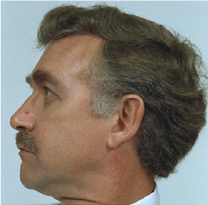
\includegraphics[width=\columnwidth]{figures/face1.png}
        \end{subfigure}
        \hfill
        \begin{subfigure}[b]{0.24\columnwidth}
            \centering
            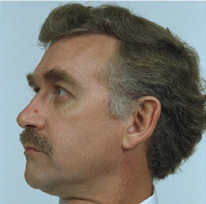
\includegraphics[width=\columnwidth]{figures/face2.png}
        \end{subfigure}
        \hfill
        \begin{subfigure}[b]{0.24\columnwidth}
            \centering
            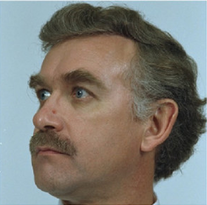
\includegraphics[width=\columnwidth]{figures/face3.png}
        \end{subfigure}
        \hfill
        \begin{subfigure}[b]{0.24\columnwidth}
            \centering
            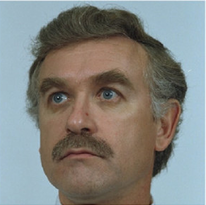
\includegraphics[width=\columnwidth]{figures/face4.png}
        \end{subfigure}
        \caption{Source: \cite{faces}}
        \label{fig:rotation}
    \end{figure}
    }}

    \only<3>{
    \begin{figure}[hb]
        \centering
            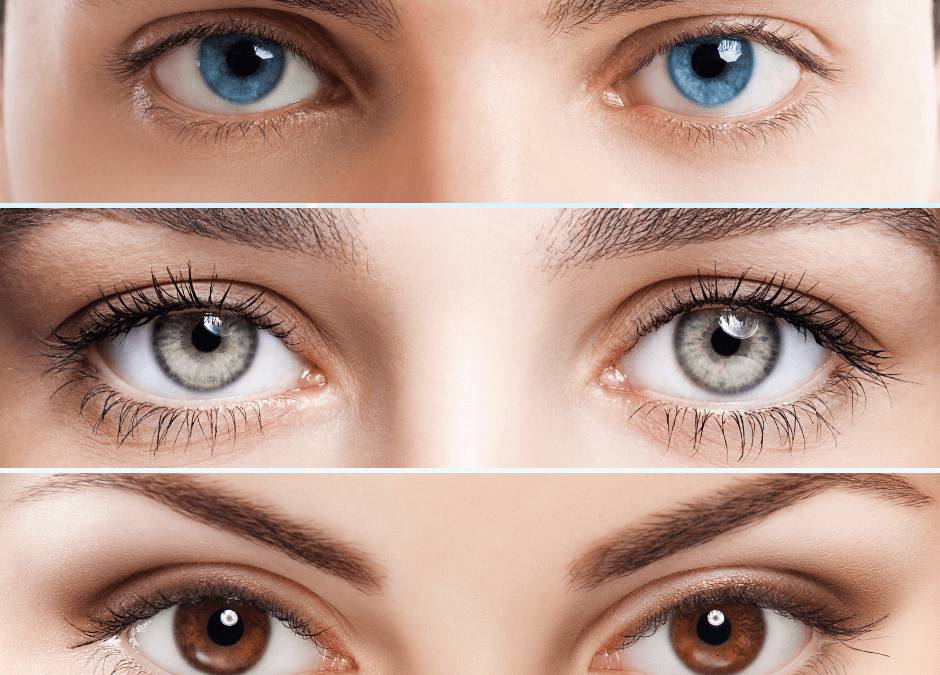
\includegraphics[width=0.5\columnwidth]{figures/eyes.png}
            \caption{Source: \href{https://valleyeyecareaz.com/how-is-your-eye-color-determined/}{valleyeyecareaz.com}}
        \label{fig:eyes}
    \end{figure}
    }

    \only<4>{
    \begin{figure}[hb]
        \centering
            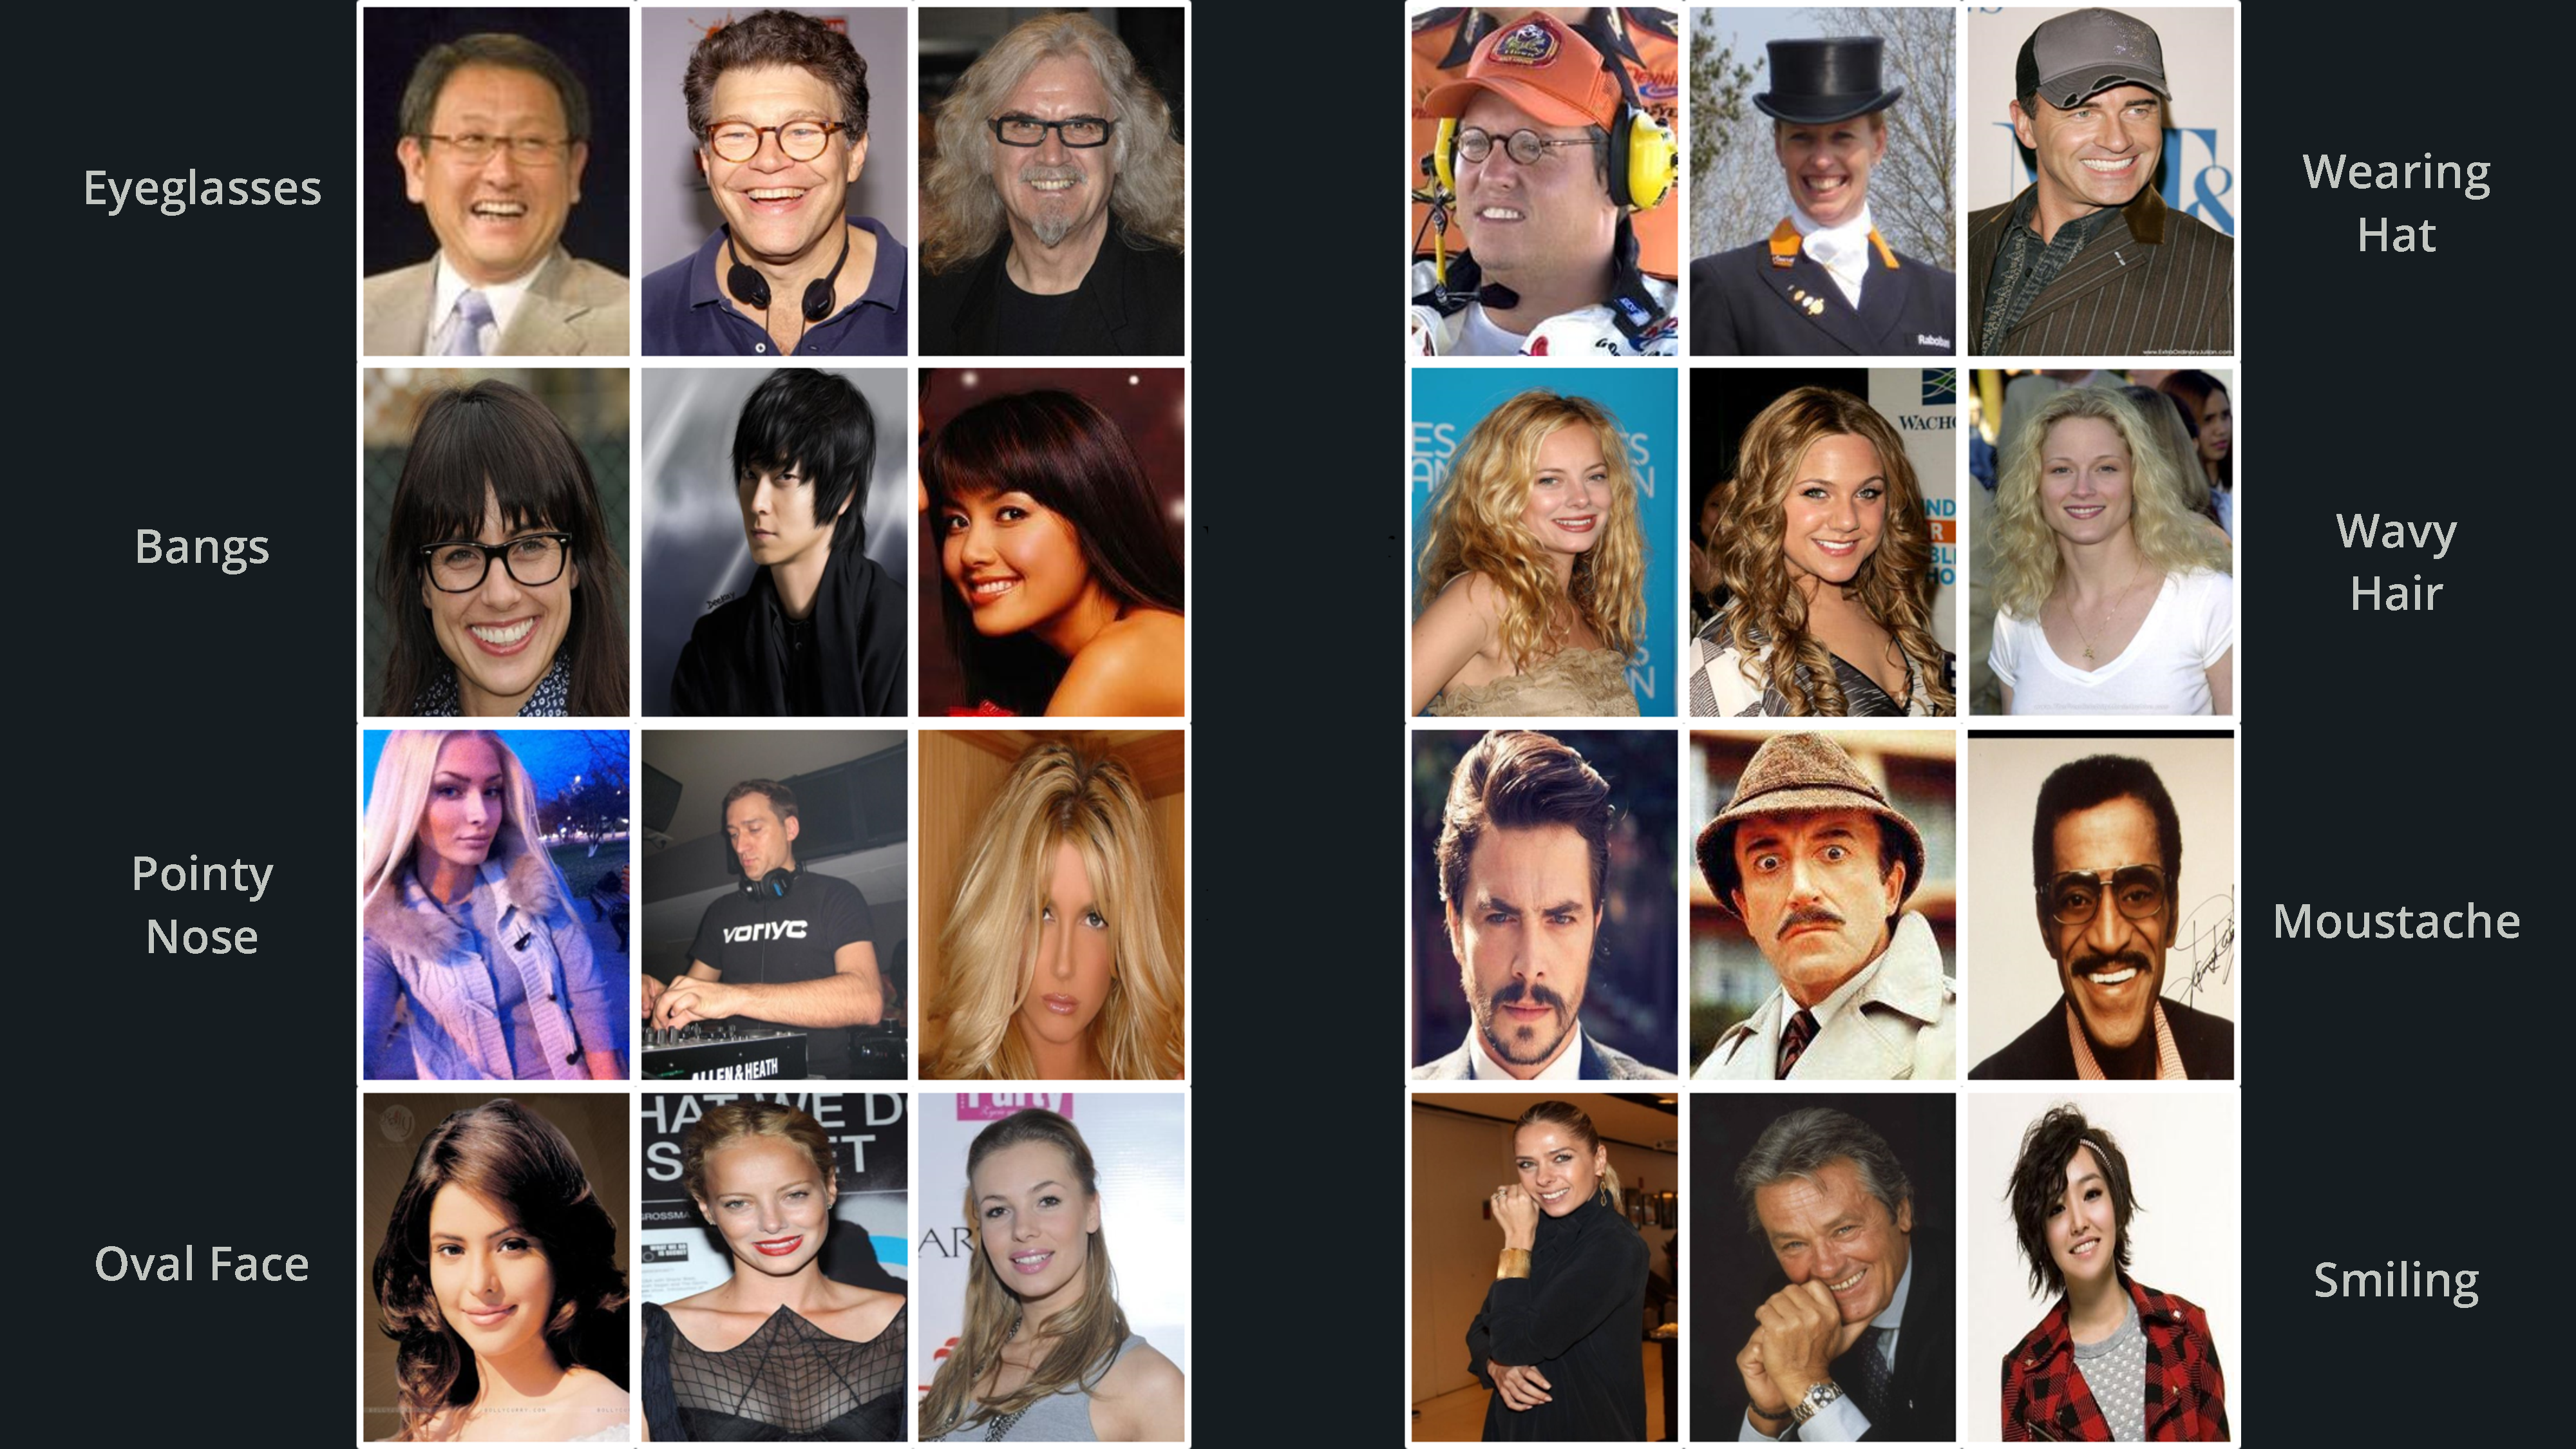
\includegraphics[width=0.6\columnwidth]{figures/celeba_bg.pdf}
            \caption{Source: \cite{liu2015faceattributes}}
        \label{fig:eyes}
    \end{figure}
    }

\end{frame}

\begin{frame}
    \frametitle{Training Discrete or Structured Latent Variable Models}
    \fontsize{12pt}{15}\selectfont

    \begin{columns}
    \hspace{2mm}\vspace{-1cm}\begin{column}{0.7\columnwidth}\vspace{-1cm}
    \begin{itemize}
        \uncover<1->{\item[] Latent variable $z$ can be }\uncover<2->{{\color{tPeony} discrete}}\uncover<3->{ or {\color{tVividBlue} structured}}
    \end{itemize}

    \begin{itemize}
        \uncover<4->{\item[] $\pi(z | x, \theta)$: distribution over possible $z$}
    \end{itemize}

    % besides this, there's also
    \begin{itemize}
        \uncover<7->{\item[] $\ell(x, z; \theta)$: downstream loss: ELBO, Log-Likelihood, (...)}
    \end{itemize}

    \end{column}

    \begin{column}{0.25\columnwidth}
            \vspace{-0.5cm}
            \begin{center}
                \begin{figure}[ht]
                \begin{tikzpicture}
                    % DISCRETE
                    \uncover<2->{\draw[draw=tPink,fill=tPink] (1.4,2) circle (0.2) node[anchor=south, yshift=2mm] {{\visible<5->{\color{tPeony} \small 0.2}}};}
                    \uncover<2->{\draw[draw=tSlateBlue,fill=tSlateBlue] (2,2) circle (0.2) node[anchor=south, yshift=2mm] {{\visible<5->{\color{tPeony} \small 0.6}}};}
                    \uncover<2->{\draw[draw=tGreen,fill=tGreen] (2.6,2) circle (0.2) node[anchor=south, yshift=2mm] {{\visible<5->{\color{tPeony} \small 0.1}}};}

                    % STRUCTURE
                    \uncover<3->{\draw[draw=tSlateBlue,fill=tSlateBlue] (1.4,1) circle (0.2) node[anchor=east, xshift=-2mm] {$[$};}
                    \uncover<3->{\draw[draw=tGreen,fill=tGreen] (2,1) circle (0.2);}
                    \uncover<3->{\draw[draw=tPink,fill=tPink] (2.6,1) circle (0.2)
                        node[anchor=west, xshift=2mm] {$]$}
                        node[anchor=west, xshift=5mm] {{\visible<6->{\color{tVividBlue} \small 0.4}}};}

                    \uncover<3->{\draw[draw=tPink,fill=tPink] (1.4,0.5) circle (0.2) node[anchor=east, xshift=-2mm] {$[$};}
                    \uncover<3->{\draw[draw=tSlateBlue,fill=tSlateBlue] (2,0.5) circle (0.2) node[anchor=north, yshift=-4mm] {\large \bf $\ldots$};}
                    \uncover<3->{\draw[draw=tGreen,fill=tGreen] (2.6,0.5) circle (0.2)
                        node[anchor=west, xshift=2mm] {$]$}
                        node[anchor=west, xshift=5mm] {{\visible<6->{\color{tVividBlue} \small 0.05}}};}

                    \uncover<3->{\draw[draw=tGreen,fill=tGreen] (1.4,-0.5) circle (0.2) node[anchor=east, xshift=-2mm] {$[$};}
                    \uncover<3->{\draw[draw=tSlateBlue,fill=tSlateBlue] (2,-0.5) circle (0.2);}
                    \uncover<3->{\draw[draw=tPink,fill=tPink] (2.6,-0.5) circle (0.2)
                        node[anchor=west, xshift=2mm] {$]$}
                        node[anchor=west, xshift=5mm] {{\visible<6->{\color{tVividBlue} \small 0.3}}};}
                \end{tikzpicture}
                \end{figure}
            \end{center}
    \end{column}
    \end{columns}

    \vspace{-0.5cm}

    \begin{itemize}
        \uncover<8->{\item[] To train, we need to compute the following expectation:}
    \end{itemize}

    \begin{equation*}\label{eq:fit}
        \uncover<9->{\mathcal{L}_{x}(\theta) =
        \sum_{z \in \mathcal Z}
        \pi(z | x, \theta)
        ~\ell(x, z; \theta)}
    \end{equation*}

    \begin{itemize}
        \uncover<10->
        {\item[] If $\mathcal Z$ is
        \only<10>{{\color{tPeony} large}, this sum can get very expensive due to $\ell(x, z; \theta)$!\quad\emoji{oface}}
        \only<11->{{\color{tVividBlue} combinatorial}, this can be intractable to compute!\quad\emoji{oface}\enspace\emoji{oface}\enspace\emoji{oface}}}
    \end{itemize}

\end{frame}

\begin{frame}
    \frametitle{Current Solutions}
    \fontsize{12pt}{15}\selectfont

    \begin{itemize}
        \item[] If $\mathcal Z$ is large, exact gradient computation is prohibitive
    \end{itemize}

    \bigskip

    \begin{itemize}
        \uncover<2->{\item[] One option: SFE (aka REINFORCE)---unbiased but high variance}
        \uncover<3->{\item[] Another option: Gumbel-Softmax---continuous relaxation, biased estimation}
    \end{itemize}

    \bigskip

    \begin{itemize}
        \uncover<4->{\item[] New option: {\color{tPeony} use sparsity}!\quad\emoji{palms}}
    \end{itemize}

    \begin{itemize}
        \uncover<5->{\item[] no need for sampling $\rightarrow$ no variance}
        \uncover<6->{\item[] no relaxation into the continuous space}
    \end{itemize}
\end{frame}

\begin{frame}
    \frametitle{Taking a step back...}
    \fontsize{12pt}{15}\selectfont
    \begin{itemize}
        \item[] Does the expectation over possible $z$ need to be expensive?
    \end{itemize}

    \begin{align*}\label{eq:fit}
        \uncover<2->{\mathcal{L}_{x}(\theta) &=
        \sum_{z \in \mathcal Z}
        \pi(z | x, \theta)~\ell(x, z; \theta) \\&=
        \pi(z_1 | x, \theta)~\ell(x, z_1; \theta) + \pi(z_2 | x, \theta)~\ell(x, z_2; \theta) + \ldots \\&+ \pi(z_{\mathrlap{i}\hphantom{1}} | x, \theta)~\ell(x, z_{\mathrlap{i}\hphantom{1}}; \theta) + \ldots + \pi(z_N | x, \theta)~\ell(x, z_N; \theta)
        }
    \end{align*}

    % \begin{itemize}
    %     \uncover<3->{\item[] If components of $\pi(z | x, \theta)$ were exactly $0$, we could skip lots of computations!}
    % \end{itemize}

    \begin{itemize}
        \uncover<3->{\item[] Usually we normalize $\pi$ with $\text{softmax} \propto \exp(s) \Rightarrow \pi(z_{\mathrlap{i}\hphantom{1}} | x, \theta)>0$}
    \end{itemize}
\end{frame}

\begin{frame}
    \frametitle{Sparse normalizers}
    \fontsize{12pt}{10}\selectfont
    \cornercite[north east]{sparsemax, sparsemap}
    \begin{itemize}
        \item[] We use {\color{tPeony} sparsemax}, {\color{tVividBlue} top-$k$ sparsemax} and {\color{tVividBlue} SparseMAP} to allow efficient marginalization
    \end{itemize}

    \begin{itemize}
        \uncover<2->{\item[] These functions are able to assign {\bf probabilities of exactly zero}!}
    \end{itemize}

    \begin{align*}
        \uncover<3->{\mathcal{L}_{x}(\theta) &=
        \sum_{z \in \mathcal Z}
        \pi(z | x, \theta)~\ell(x, z; \theta) \\&=
        \pi(z_1 | x, \theta)~\ell(x, z_1; \theta) + \alt<3>{\underbrace{\pi(z_2 | x, \theta)}_{=0}~\ell(x, z_2; \theta)}{\cancel{\underbrace{\pi(z_2 | x, \theta)}_{=0}~\ell(x, z_2; \theta)}} + \ldots \\&+
        \pi(z_{\mathrlap{i}\hphantom{1}} | x, \theta)~\ell(x, z_{\mathrlap{i}\hphantom{1}}; \theta) + \ldots + \alt<3>{\underbrace{\pi(z_N | x, \theta)}_{=0}~\ell(x, z_N; \theta)}{\cancel{\underbrace{\pi(z_N | x, \theta)}_{=0}~\ell(x, z_N; \theta)}}
        }
    \end{align*}

    \begin{itemize}
        \uncover<4->{\item[] No need for computing $\ell(x, z; \theta)$ for all $z \in \mathcal Z$!}
    \end{itemize}
\end{frame}

\begin{frame}[label=blub]
    \frametitle{Discrete, unstructured case: sparsemax}
    \begin{columns}
    \begin{column}{.58\textwidth}
    \centering
    \vspace{-.3cm}
    \[ \mapo(s) = \argmax_{\p\in\triangle} \p^\top s - \Omega(\p) \]
    \vspace{-.3cm}
    {
    \fontsize{12.5pt}{13}\selectfont%
    \def\vph{\vphantom{$\sum_j$}}
    \renewcommand{\arraystretch}{2}
    \begin{tabular}{r@{~}r@{:~~}r@{$\,=\,$}l}
    \onslide<2->{
    \colorbul{colorArgmax} &
    argmax    & $\Omega(\p)$ & \vph $0$
    \textcolor{mygr}{\emph{(no smoothing)}} \\}
    \onslide<3->{
    \colorbul{colorSoftmax} &
    softmax   & $\Omega(\p)$ & $\sum_j p_j \log p_j$ \\}
    \onslide<4->{
    \colorbul{colorSparsemax} &
    sparsemax & $\Omega(\p)$ & \vph $\nicefrac{1}{2} \|\p\|^2_2$ \\}
    \end{tabular}%
    }
    \end{column}%
    %
    %
    \begin{column}{.42\textwidth}
    \centering
    % BEGIN softmax 2d plot
    \begin{tikzpicture}[scale=.9]
        \draw[axisline,->] (3, 3) -- (3, 5.5) node[left] {$p_1$};
        \draw[axisline,->] (3, 3) -- (7, 3) node[right]{$\theta_1$};
    
        \node[axislabel,left] at (3, 3) {$0$};
        \node[axislabel,left] at (3, 5) {$1$};
    
        \draw[axisline] ($(3,3) + (-\ticksize, 0)$) -- ($(3,3) + (+\ticksize, 0)$);
        \draw[axisline] ($(3,4) + (-\ticksize, 0)$) -- ($(3,4) + (+\ticksize, 0)$);
        \draw[axisline] ($(3,5) + (-\ticksize, 0)$) -- ($(3,5) + (+\ticksize, 0)$);
    
        \draw[axisline] ($(3,3) + (0, -\ticksize)$) -- ($(3,3) + (0, +\ticksize)$);
        \draw[axisline] ($(4,3) + (0, -\ticksize)$) -- ($(4,3) + (0, +\ticksize)$);
        \draw[axisline] ($(5,3) + (0, -\ticksize)$) -- ($(5,3) + (0, +\ticksize)$);
        \draw[axisline] ($(6,3) + (0, -\ticksize)$) -- ($(6,3) + (0, +\ticksize)$);
    
        \node[axislabel,below] at (4, 3) {$-1$};
        \node[axislabel,below] at (5, 3) {$0$};
        \node[axislabel,below] at (6, 3) {$1$};
    
        \onslide<2->{
            \draw[ultra thick,colorArgmax] (3, 3) -- (5,3) ;
            \draw[ultra thick,colorArgmax] (5, 5) -- (7,5) ;
        }
        \onslide<3->{
            \draw (3, 3.1)
            edge[colorSoftmax,ultra thick,out=360,in=180,looseness=1.5] (7, 4.9);
        }
        \onslide<4->{
            \draw[ultra thick,colorSparsemax,dashed]
            (3, 3) -- (4,3) -- (6,5) -- (7, 5) ;
        }
    \end{tikzpicture}%
    % END softmax 2d plot
    \\[-0.1cm]
    % BEGIN Simplex barycentric
    \begin{tikzpicture}
    \setupsimplexbary{}
    \coordinate (argmax)    at (barycentric cs:L1=0,L2=0,L3=1);
    \coordinate (softmax)   at (barycentric cs:L1=.3,L2=.2,L3=.5);
    \coordinate (sparsemax) at (barycentric cs:L1=.3,L2=0,L3=.7);
    
    \onslide<2->{
    \node[label=west:{\small $[0,0,1]$}] at (argmax) {};
    \draw[point,fill=colorArgmax] (argmax) circle[radius=5pt];
    }
    \onslide<3->{
    \node[label=south:{\small $[.3,.2,.5]$}] at (softmax) {};
    \draw[point,fill=colorSoftmax] (softmax) circle[radius=5pt];
    }
    \onslide<4->{
    \node[label=west:{\small $[.3,0,.7]$}] at (sparsemax) {};
    \draw[point,fill=colorSparsemax] (sparsemax) circle[radius=5pt];
    }
    \end{tikzpicture}%
    %% END Simplex Barycentric
    \vspace{-.5cm}%
    \end{column}%
    \end{columns}%
        
    \begin{tikzpicture}[font=\footnotesize,remember picture,overlay]
        \node[anchor=north east] at (current page.north east) {
            \citep{sparseattn}};
        \node<4>[anchor=south west] at (current page.south west) {
            \citep{sparsemax}};
    \end{tikzpicture}
\end{frame}

\begin{frame}
    \frametitle{Semi-Supervised VAE}\cornerciteme{sparsemarg}

    \newcommand*\parcolor{myfg}
    \newcommand*\clfcolor{myfg}
    \newcommand*\colParseZero{mybg}
    \newcommand*\colParseNonz{mybg}
    \only<1->{
    \renewcommand*\parcolor{tPeony}
    \renewcommand*\clfcolor{tYellow}
    }
    \begin{align*}
        \mathcal{L}_{x}(\theta) &=
            \tikzmark{sum}\sum_{z \in \mathcal{Z}}
            \textcolor{\parcolor}{\pi\tikzmark{parp}(z | x)}~
            \textcolor{\clfcolor}{\ell\tikzmark{clfp}(x, z)}\\
            &= \mathbb{E}_{z \sim \textcolor{\parcolor}{\pi(z | x)}}~%
            \textcolor{\clfcolor}{\ell(x, z)}
    \end{align*}

    \vspace{\baselineskip}
    \small
    \begin{itemize}
    \item<2-> Semi-Supervised VAE on MNIST: $z$ is a possible digit
    \item<3-> Train this with 10\% labeled data
    \end{itemize}
    \begin{tikzpicture}[%
        remember picture,
        overlay,
        expl/.style={font=\small}]
    \uncover<2->{
        \node[expl,anchor=north east] (explpar)
            at ($(current page.north east) - (.5, 1.5)$)
            {Gaussian VAE};
        \path (explpar.west) edge[->,very thick,bend right] ([yshift=1.5ex]{pic cs:clfp});
    }
    %
    \uncover<3->{
        \node[expl,anchor=north west,align=left] (explsum)
            at ($(current page.west) + (.5, -1.5)$)
            {sum over \\ the 10 digits};
        \path (explsum.east) edge[->,very thick,bend left] ([yshift=2.5ex]{pic cs:sum});
    }
    \uncover<2->{
        \node[expl,anchor=north east,align=right] (explscore)
            at ($(current page.north east) - (.5, 4)$)
            {discrete inference network};
        \path (explscore.south west) edge[->,very thick,bend left] ([yshift=-.5ex]{pic cs:parp});
    }
    \end{tikzpicture}
\end{frame}

\begin{frame}
    \frametitle{Semi-Supervised VAE}
    \begin{columns}[T]
    \begin{column}{.53\textwidth}
        \centering\small%
        \begin{tabular}{lrr}
            \toprule
            Method &
            Accuracy (\%)
            & Dec. calls\\
            \midrule
        \multicolumn{3}{l}{\emph{Monte Carlo}} \\
            SFE
            & $94.75${\tiny\color{gray}$\pm .002$} & $1$ \\
            SFE$+$
            & $96.53${\tiny\color{gray}$\pm .001$}  & $2$  \\
            NVIL
            & $96.01${\tiny\color{gray}$\pm .002$}  & $1$  \\
            Gumbel
            & $95.46${\tiny\color{gray}$\pm .001$}  & $1$  \\
            \midrule
        \multicolumn{3}{l}{\emph{Marginalization}} \\
            Dense
            & $96.93${\tiny\color{gray}$\pm .001$}  & $10$  \\
            Sparse {\small \color{gray}{(proposed)}}
            & $96.87${\tiny\color{gray}$\pm .001$}  & $1.01${\tiny\color{gray}$\pm 0.01$}  \\
            \bottomrule
            \end{tabular}
    \end{column}
    \begin{column}{.47\textwidth}
        \fontsize{10pt}{10}\selectfont\centering%
        \onslide<4->{
        % This file was created by tikzplotlib v0.9.4.
\small
\begin{tikzpicture}

\definecolor{color0}{rgb}{0.894117647058824,0.101960784313725,0.109803921568627}
\definecolor{color1}{rgb}{1,0.498039215686275,0}
\definecolor{color2}{rgb}{0.968627450980392,0.505882352941176,0.749019607843137}
\definecolor{color3}{rgb}{0.215686274509804,0.494117647058824,0.72156862745098}
\definecolor{color4}{rgb}{0.870588235294118,0.870588235294118,0}

\begin{axis}[
scale=.75,
legend cell align={left},
legend style={fill opacity=0.1, draw opacity=1, text opacity=1},
tick align=outside,
tick pos=left,
x grid style={white!69.0196078431373!black},
xlabel={Epoch},
xmin=1, xmax=202,
xtick style={color=black},
y grid style={white!69.0196078431373!black},
ylabel={Negative ELBO},
ymin=97.1, ymax=105.5,
ytick style={color=black}
]
\path [draw=color0, line width=1pt]
(axis cs:0,110.571628222803)
--(axis cs:0,110.616042675635);

\path [draw=color0, line width=1pt]
(axis cs:5,105.62209213224)
--(axis cs:5,105.704893036217);

\path [draw=color0, line width=1pt]
(axis cs:10,104.289450185493)
--(axis cs:10,104.356994516656);

\path [draw=color0, line width=1pt]
(axis cs:15,103.407209298477)
--(axis cs:15,103.476579764023);

\path [draw=color0, line width=1pt]
(axis cs:20,102.773344218468)
--(axis cs:20,102.825509846474);

\path [draw=color0, line width=1pt]
(axis cs:25,102.213106343832)
--(axis cs:25,102.282459452066);

\path [draw=color0, line width=1pt]
(axis cs:30,101.725467036023)
--(axis cs:30,101.820451237903);

\path [draw=color0, line width=1pt]
(axis cs:35,101.245988632048)
--(axis cs:35,101.334083389436);

\path [draw=color0, line width=1pt]
(axis cs:40,100.909448112661)
--(axis cs:40,100.97308362562);

\path [draw=color0, line width=1pt]
(axis cs:45,100.543817511853)
--(axis cs:45,100.626635369007);

\path [draw=color0, line width=1pt]
(axis cs:50,100.299712409677)
--(axis cs:50,100.380463371573);

\path [draw=color0, line width=1pt]
(axis cs:55,99.9914284050014)
--(axis cs:55,100.074857300565);

\path [draw=color0, line width=1pt]
(axis cs:60,99.9003536552268)
--(axis cs:60,100.007995954148);

\path [draw=color0, line width=1pt]
(axis cs:65,99.704677941787)
--(axis cs:65,99.7719318604591);

\path [draw=color0, line width=1pt]
(axis cs:70,99.512591227806)
--(axis cs:70,99.6056003005144);

\path [draw=color0, line width=1pt]
(axis cs:75,99.2968394860584)
--(axis cs:75,99.3603535071057);

\path [draw=color0, line width=1pt]
(axis cs:80,99.1895523660352)
--(axis cs:80,99.3006438619921);

\path [draw=color0, line width=1pt]
(axis cs:85,99.0947624008693)
--(axis cs:85,99.1854026992284);

\path [draw=color0, line width=1pt]
(axis cs:90,98.9419574019052)
--(axis cs:90,99.0291546586417);

\path [draw=color0, line width=1pt]
(axis cs:95,98.7685936844909)
--(axis cs:95,98.8469992720521);

\path [draw=color0, line width=1pt]
(axis cs:100,98.6924243915877)
--(axis cs:100,98.7649715434708);

\path [draw=color0, line width=1pt]
(axis cs:105,98.6493410445112)
--(axis cs:105,98.7355893754106);

\path [draw=color0, line width=1pt]
(axis cs:110,98.4847570378102)
--(axis cs:110,98.5481546443187);

\path [draw=color0, line width=1pt]
(axis cs:115,98.3900102720628)
--(axis cs:115,98.4639402284255);

\path [draw=color0, line width=1pt]
(axis cs:120,98.4279693596278)
--(axis cs:120,98.5433822639073);

\path [draw=color0, line width=1pt]
(axis cs:125,98.2681371217175)
--(axis cs:125,98.3506113524036);

\path [draw=color0, line width=1pt]
(axis cs:130,98.2755771208057)
--(axis cs:130,98.3637051057568);

\path [draw=color0, line width=1pt]
(axis cs:135,98.1519624650895)
--(axis cs:135,98.244399839598);

\path [draw=color0, line width=1pt]
(axis cs:140,98.1250063491776)
--(axis cs:140,98.2095242904708);

\path [draw=color0, line width=1pt]
(axis cs:145,97.9583158375388)
--(axis cs:145,98.0694994090433);

\path [draw=color0, line width=1pt]
(axis cs:150,98.0437309578043)
--(axis cs:150,98.1430503532309);

\path [draw=color0, line width=1pt]
(axis cs:155,97.9080906432997)
--(axis cs:155,98.0325358825793);

\path [draw=color0, line width=1pt]
(axis cs:160,97.9438041674736)
--(axis cs:160,97.9982872021553);

\path [draw=color0, line width=1pt]
(axis cs:165,97.7717692124589)
--(axis cs:165,97.8538380873458);

\path [draw=color0, line width=1pt]
(axis cs:170,97.7947733818513)
--(axis cs:170,97.9104039252776);

\path [draw=color0, line width=1pt]
(axis cs:175,97.7514530083922)
--(axis cs:175,97.8663829901429);

\path [draw=color0, line width=1pt]
(axis cs:180,97.7297998759255)
--(axis cs:180,97.804909291555);

\path [draw=color0, line width=1pt]
(axis cs:185,97.6381521365036)
--(axis cs:185,97.7025918820511);

\path [draw=color0, line width=1pt]
(axis cs:190,97.6893112699308)
--(axis cs:190,97.8114165743075);

\path [draw=color0, line width=1pt]
(axis cs:195,97.530511048186)
--(axis cs:195,97.6161030265211);

\path [draw=color0, line width=1pt]
(axis cs:200,97.6454695308675)
--(axis cs:200,97.7513017093669);

\path [draw=color1, thick]
(axis cs:0,110.627656081213)
--(axis cs:0,110.677801987635);

\path [draw=color1, thick]
(axis cs:5,105.706752241274)
--(axis cs:5,105.865315019468);

\path [draw=color1, thick]
(axis cs:10,104.251092751157)
--(axis cs:10,104.39130837189);

\path [draw=color1, thick]
(axis cs:15,103.02386310639)
--(axis cs:15,103.129296988825);

\path [draw=color1, thick]
(axis cs:20,102.185802869572)
--(axis cs:20,102.311458177791);

\path [draw=color1, thick]
(axis cs:25,101.498045278342)
--(axis cs:25,101.599491953103);

\path [draw=color1, thick]
(axis cs:30,101.074134287995)
--(axis cs:30,101.195169606048);

\path [draw=color1, thick]
(axis cs:35,100.688277085196)
--(axis cs:35,100.794839064706);

\path [draw=color1, thick]
(axis cs:40,100.470196032671)
--(axis cs:40,100.584731030317);

\path [draw=color1, thick]
(axis cs:45,100.114440390114)
--(axis cs:45,100.257237771508);

\path [draw=color1, thick]
(axis cs:50,99.8929637508349)
--(axis cs:50,99.9790409488721);

\path [draw=color1, thick]
(axis cs:55,99.4751854380556)
--(axis cs:55,99.6703162709288);

\path [draw=color1, thick]
(axis cs:60,99.4392706157917)
--(axis cs:60,99.6078973529582);

\path [draw=color1, thick]
(axis cs:65,99.2057001296773)
--(axis cs:65,99.3453481491313);

\path [draw=color1, thick]
(axis cs:70,99.139523129024)
--(axis cs:70,99.2743074373822);

\path [draw=color1, thick]
(axis cs:75,99.0585529362254)
--(axis cs:75,99.1688610042043);

\path [draw=color1, thick]
(axis cs:80,98.863532244795)
--(axis cs:80,98.9907447937792);

\path [draw=color1, thick]
(axis cs:85,98.6890531083094)
--(axis cs:85,98.791636894132);

\path [draw=color1, thick]
(axis cs:90,98.6046054723124)
--(axis cs:90,98.7568752405782);

\path [draw=color1, thick]
(axis cs:95,98.5015275966912)
--(axis cs:95,98.6355482089728);

\path [draw=color1, thick]
(axis cs:100,98.5031524382435)
--(axis cs:100,98.6100830353893);

\path [draw=color1, thick]
(axis cs:105,98.4936773624417)
--(axis cs:105,98.6237222347263);

\path [draw=color1, thick]
(axis cs:110,98.3101249716939)
--(axis cs:110,98.4445198036967);

\path [draw=color1, thick]
(axis cs:115,98.427620263025)
--(axis cs:115,98.5260891485961);

\path [draw=color1, thick]
(axis cs:120,98.2365748731903)
--(axis cs:120,98.3342777879425);

\path [draw=color1, thick]
(axis cs:125,98.2255084713109)
--(axis cs:125,98.38844111365);

\path [draw=color1, thick]
(axis cs:130,98.1163595550203)
--(axis cs:130,98.2660211212493);

\path [draw=color1, thick]
(axis cs:135,98.0937488614553)
--(axis cs:135,98.2127208651072);

\path [draw=color1, thick]
(axis cs:140,98.0585679595026)
--(axis cs:140,98.1632795746771);

\path [draw=color1, thick]
(axis cs:145,98.1005616053344)
--(axis cs:145,98.2021132603883);

\path [draw=color1, thick]
(axis cs:150,98.029635259175)
--(axis cs:150,98.1676334175828);

\path [draw=color1, thick]
(axis cs:155,98.0933789691696)
--(axis cs:155,98.1758226909867);

\path [draw=color1, thick]
(axis cs:160,97.9562209316475)
--(axis cs:160,98.0729889682549);

\path [draw=color1, thick]
(axis cs:165,97.949017347317)
--(axis cs:165,98.0935470447728);

\path [draw=color1, thick]
(axis cs:170,97.8620924517951)
--(axis cs:170,97.9806428387322);

\path [draw=color1, thick]
(axis cs:175,97.9098973693818)
--(axis cs:175,98.0343851623565);

\path [draw=color1, thick]
(axis cs:180,97.8642887851381)
--(axis cs:180,98.0409861782408);

\path [draw=color1, thick]
(axis cs:185,97.766666124376)
--(axis cs:185,97.9967158336318);

\path [draw=color1, thick]
(axis cs:190,97.788889657506)
--(axis cs:190,97.8705555329237);

\path [draw=color1, thick]
(axis cs:195,97.7695971257876)
--(axis cs:195,97.8705502741148);

\path [draw=color1, thick]
(axis cs:200,97.676539048256)
--(axis cs:200,97.8900106343612);

\path [draw=color2, thick]
(axis cs:0,110.667671743089)
--(axis cs:0,110.722681650465);

\path [draw=color2, thick]
(axis cs:5,106.483563798014)
--(axis cs:5,106.755126387533);

\path [draw=color2, thick]
(axis cs:10,105.265325161184)
--(axis cs:10,105.615572360788);

\path [draw=color2, thick]
(axis cs:15,104.528087390467)
--(axis cs:15,104.730024181799);

\path [draw=color2, thick]
(axis cs:20,103.768548703352)
--(axis cs:20,103.906315493426);

\path [draw=color2, thick]
(axis cs:25,103.117035642729)
--(axis cs:25,103.338207277193);

\path [draw=color2, thick]
(axis cs:30,102.790858085322)
--(axis cs:30,102.949431221319);

\path [draw=color2, thick]
(axis cs:35,102.420181417919)
--(axis cs:35,102.692468118214);

\path [draw=color2, thick]
(axis cs:40,101.953505979879)
--(axis cs:40,102.11779834141);

\path [draw=color2, thick]
(axis cs:45,101.605904790239)
--(axis cs:45,101.75691717021);

\path [draw=color2, thick]
(axis cs:50,101.470575734144)
--(axis cs:50,101.61874616527);

\path [draw=color2, thick]
(axis cs:55,101.197271375808)
--(axis cs:55,101.416739244309);

\path [draw=color2, thick]
(axis cs:60,100.910259467554)
--(axis cs:60,101.06691033225);

\path [draw=color2, thick]
(axis cs:65,100.811883301745)
--(axis cs:65,101.000802855481);

\path [draw=color2, thick]
(axis cs:70,100.628725831965)
--(axis cs:70,100.885245115301);

\path [draw=color2, thick]
(axis cs:75,100.324332760492)
--(axis cs:75,100.442026187261);

\path [draw=color2, thick]
(axis cs:80,100.178942312571)
--(axis cs:80,100.475639901784);

\path [draw=color2, thick]
(axis cs:85,99.9694360453458)
--(axis cs:85,100.165645436588);

\path [draw=color2, thick]
(axis cs:90,99.7062381923905)
--(axis cs:90,99.9938823520431);

\path [draw=color2, thick]
(axis cs:95,99.782874624705)
--(axis cs:95,99.8487354827169);

\path [draw=color2, thick]
(axis cs:100,99.6613457276373)
--(axis cs:100,99.7565757201167);

\path [draw=color2, thick]
(axis cs:105,99.4611038629233)
--(axis cs:105,99.5586761053385);

\path [draw=color2, thick]
(axis cs:110,99.4817789142452)
--(axis cs:110,99.6602132732548);

\path [draw=color2, thick]
(axis cs:115,99.3468294377173)
--(axis cs:115,99.4159482722436);

\path [draw=color2, thick]
(axis cs:120,99.141580926534)
--(axis cs:120,99.271195257548);

\path [draw=color2, thick]
(axis cs:125,99.1192806472576)
--(axis cs:125,99.2834537277424);

\path [draw=color2, thick]
(axis cs:130,99.0235558578023)
--(axis cs:130,99.1700354507914);

\path [draw=color2, thick]
(axis cs:135,99.1761870048272)
--(axis cs:135,99.532272467829);

\path [draw=color2, thick]
(axis cs:140,99.1153352177682)
--(axis cs:140,99.2472807490287);

\path [draw=color2, thick]
(axis cs:145,98.7532872367982)
--(axis cs:145,98.8955485175963);

\path [draw=color2, thick]
(axis cs:150,98.8283402895275)
--(axis cs:150,98.9566206479725);

\path [draw=color2, thick]
(axis cs:155,98.768272445518)
--(axis cs:155,98.8687789460836);

\path [draw=color2, thick]
(axis cs:160,98.8125847348663)
--(axis cs:160,98.9838111391571);

\path [draw=color2, thick]
(axis cs:165,98.5870355780569)
--(axis cs:165,98.7299962822946);

\path [draw=color2, thick]
(axis cs:170,98.5641170271013)
--(axis cs:170,98.7153095476057);

\path [draw=color2, thick]
(axis cs:175,98.5214131010244)
--(axis cs:175,98.702083908253);

\path [draw=color2, thick]
(axis cs:180,98.3888573706301)
--(axis cs:180,98.488860219702);

\path [draw=color2, thick]
(axis cs:185,98.3901603236432)
--(axis cs:185,98.620610855556);

\path [draw=color2, thick]
(axis cs:190,98.4326878189535)
--(axis cs:190,98.6290248275309);

\path [draw=color2, thick]
(axis cs:195,98.3281897838033)
--(axis cs:195,98.5063866322123);

\path [draw=color2, thick]
(axis cs:200,98.3254687617908)
--(axis cs:200,98.4676388431897);

\path [draw=color3, thick]
(axis cs:0,110.602628549784)
--(axis cs:0,110.654276052266);

\path [draw=color3, thick]
(axis cs:5,105.976421191421)
--(axis cs:5,106.086629650864);

\path [draw=color3, thick]
(axis cs:10,104.686016970886)
--(axis cs:10,104.733898800599);

\path [draw=color3, thick]
(axis cs:15,103.722053944156)
--(axis cs:15,103.865365184262);

\path [draw=color3, thick]
(axis cs:20,103.028494114149)
--(axis cs:20,103.116822963487);

\path [draw=color3, thick]
(axis cs:25,102.6033735088)
--(axis cs:25,102.73937246288);

\path [draw=color3, thick]
(axis cs:30,101.982135306812)
--(axis cs:30,102.062316597485);

\path [draw=color3, thick]
(axis cs:35,101.56680058494)
--(axis cs:35,101.653621778342);

\path [draw=color3, thick]
(axis cs:40,101.228760366328)
--(axis cs:40,101.308081979864);

\path [draw=color3, thick]
(axis cs:45,100.91559693553)
--(axis cs:45,101.09211790822);

\path [draw=color3, thick]
(axis cs:50,100.715529800361)
--(axis cs:50,100.781035446221);

\path [draw=color3, thick]
(axis cs:55,100.284129784015)
--(axis cs:55,100.401266028973);

\path [draw=color3, thick]
(axis cs:60,100.136854336586)
--(axis cs:60,100.240103366051);

\path [draw=color3, thick]
(axis cs:65,99.8551212918418)
--(axis cs:65,99.9795039522988);

\path [draw=color3, thick]
(axis cs:70,99.7252302427781)
--(axis cs:70,99.8387315492141);

\path [draw=color3, thick]
(axis cs:75,99.5236912911197)
--(axis cs:75,99.6395121390561);

\path [draw=color3, thick]
(axis cs:80,99.4197217550092)
--(axis cs:80,99.5033083353228);

\path [draw=color3, thick]
(axis cs:85,99.3302764392952)
--(axis cs:85,99.4162308238884);

\path [draw=color3, thick]
(axis cs:90,99.1285783522856)
--(axis cs:90,99.1683592087495);

\path [draw=color3, thick]
(axis cs:95,98.9709728146841)
--(axis cs:95,99.0789615725229);

\path [draw=color3, thick]
(axis cs:100,98.8787928184983)
--(axis cs:100,99.0089269080642);

\path [draw=color3, thick]
(axis cs:105,98.8716916737113)
--(axis cs:105,99.0200563731637);

\path [draw=color3, thick]
(axis cs:110,98.7279148782457)
--(axis cs:110,98.8484721456801);

\path [draw=color3, thick]
(axis cs:115,98.6767164317005)
--(axis cs:115,98.7957170399792);

\path [draw=color3, thick]
(axis cs:120,98.5780803608091)
--(axis cs:120,98.6203907085269);

\path [draw=color3, thick]
(axis cs:125,98.4521045701371)
--(axis cs:125,98.5314693434371);

\path [draw=color3, thick]
(axis cs:130,98.3776252768865)
--(axis cs:130,98.4630714394221);

\path [draw=color3, thick]
(axis cs:135,98.348839879622)
--(axis cs:135,98.4589039558272);

\path [draw=color3, thick]
(axis cs:140,98.3020782930936)
--(axis cs:140,98.3743255155002);

\path [draw=color3, thick]
(axis cs:145,98.2389102090793)
--(axis cs:145,98.3121029745145);

\path [draw=color3, thick]
(axis cs:150,98.1700772251234)
--(axis cs:150,98.2461810146227);

\path [draw=color3, thick]
(axis cs:155,98.0599698152065)
--(axis cs:155,98.1876009855747);

\path [draw=color3, thick]
(axis cs:160,98.0501097252529)
--(axis cs:160,98.1519822547276);

\path [draw=color3, thick]
(axis cs:165,97.9869192373277)
--(axis cs:165,98.1074411142348);

\path [draw=color3, thick]
(axis cs:170,97.9562103379446)
--(axis cs:170,98.054098499946);

\path [draw=color3, thick]
(axis cs:175,97.8537923449074)
--(axis cs:175,97.9198068982566);

\path [draw=color3, thick]
(axis cs:180,97.7835440487471)
--(axis cs:180,97.8533425479326);

\path [draw=color3, thick]
(axis cs:185,97.7571509252569)
--(axis cs:185,97.8370385278681);

\path [draw=color3, thick]
(axis cs:190,97.6644307218972)
--(axis cs:190,97.7558863557395);

\path [draw=color3, thick]
(axis cs:195,97.8125477291052)
--(axis cs:195,97.8993236087854);

\path [draw=color3, thick]
(axis cs:200,97.6539407705038)
--(axis cs:200,97.7391317392618);

\path [draw=color4, thick]
(axis cs:0,109.115286948018)
--(axis cs:0,109.381600259013);

\path [draw=color4, thick]
(axis cs:5,106.282004510241)
--(axis cs:5,106.442658270521);

\path [draw=color4, thick]
(axis cs:10,104.396784651101)
--(axis cs:10,104.604474198997);

\path [draw=color4, thick]
(axis cs:15,103.323337914808)
--(axis cs:15,103.482654211657);

\path [draw=color4, thick]
(axis cs:20,102.778455356846)
--(axis cs:20,103.020767970791);

\path [draw=color4, thick]
(axis cs:25,102.055643913527)
--(axis cs:25,102.23702271245);

\path [draw=color4, thick]
(axis cs:30,101.529721481467)
--(axis cs:30,101.638959853983);

\path [draw=color4, thick]
(axis cs:35,101.134941232361)
--(axis cs:35,101.228889334045);

\path [draw=color4, thick]
(axis cs:40,100.906734618429)
--(axis cs:40,101.146105042215);

\path [draw=color4, thick]
(axis cs:45,100.697209372744)
--(axis cs:45,100.824752602354);

\path [draw=color4, thick]
(axis cs:50,100.353978259345)
--(axis cs:50,100.619825451592);

\path [draw=color4, thick]
(axis cs:55,100.084291283199)
--(axis cs:55,100.24559305518);

\path [draw=color4, thick]
(axis cs:60,100.010707402261)
--(axis cs:60,100.119865107505);

\path [draw=color4, thick]
(axis cs:65,99.7864048943775)
--(axis cs:65,99.9255106940014);

\path [draw=color4, thick]
(axis cs:70,99.631284648257)
--(axis cs:70,99.7560169874852);

\path [draw=color4, thick]
(axis cs:75,99.4452606980236)
--(axis cs:75,99.624603193578);

\path [draw=color4, thick]
(axis cs:80,99.3618639961725)
--(axis cs:80,99.4920193656439);

\path [draw=color4, thick]
(axis cs:85,99.2837623633726)
--(axis cs:85,99.3978050194399);

\path [draw=color4, thick]
(axis cs:90,99.266347190475)
--(axis cs:90,99.3817576679235);

\path [draw=color4, thick]
(axis cs:95,99.3123228170201)
--(axis cs:95,99.660885801144);

\path [draw=color4, thick]
(axis cs:100,99.0990519167043)
--(axis cs:100,99.2413808225535);

\path [draw=color4, thick]
(axis cs:105,98.8874418897035)
--(axis cs:105,99.0510957079527);

\path [draw=color4, thick]
(axis cs:110,98.975193322023)
--(axis cs:110,99.2649327155746);

\path [draw=color4, thick]
(axis cs:115,98.8336393432915)
--(axis cs:115,99.0471651000678);

\path [draw=color4, thick]
(axis cs:120,98.8308258199566)
--(axis cs:120,98.9343551492817);

\path [draw=color4, thick]
(axis cs:125,98.656977400232)
--(axis cs:125,98.7910816817992);

\path [draw=color4, thick]
(axis cs:130,98.6945838969624)
--(axis cs:130,98.845497890147);

\path [draw=color4, thick]
(axis cs:135,98.6141177603053)
--(axis cs:135,98.7381649545384);

\path [draw=color4, thick]
(axis cs:140,98.5875804361404)
--(axis cs:140,98.7294895711839);

\path [draw=color4, thick]
(axis cs:145,98.6315291825926)
--(axis cs:145,98.944827323755);

\path [draw=color4, thick]
(axis cs:150,98.5094485836863)
--(axis cs:150,98.6495495242238);

\path [draw=color4, thick]
(axis cs:155,98.3895212745971)
--(axis cs:155,98.5292638206178);

\path [draw=color4, thick]
(axis cs:160,98.2698468425989)
--(axis cs:160,98.4126009723425);

\path [draw=color4, thick]
(axis cs:165,98.3838028476987)
--(axis cs:165,98.5055968715395);

\path [draw=color4, thick]
(axis cs:170,98.2593796537036)
--(axis cs:170,98.3188368990307);

\path [draw=color4, thick]
(axis cs:175,98.5055199805482)
--(axis cs:175,98.6556677635925);

\path [draw=color4, thick]
(axis cs:180,98.2703711104053)
--(axis cs:180,98.403257124458);

\path [draw=color4, thick]
(axis cs:185,98.1379741875829)
--(axis cs:185,98.2555164130031);

\path [draw=color4, thick]
(axis cs:190,98.1838837762334)
--(axis cs:190,98.3041319708369);

\path [draw=color4, thick]
(axis cs:195,98.0923628934146)
--(axis cs:195,98.204795920062);

\path [draw=color4, thick]
(axis cs:200,98.1158716660487)
--(axis cs:200,98.3141988295567);

\path [draw=white!60!black, thick]
(axis cs:0,110.590080177886)
--(axis cs:0,110.625547873871);

\path [draw=white!60!black, thick]
(axis cs:5,105.789744869155)
--(axis cs:5,105.860650333482);

\path [draw=white!60!black, thick]
(axis cs:10,104.306409792426)
--(axis cs:10,104.455569882867);

\path [draw=white!60!black, thick]
(axis cs:15,103.193854098826)
--(axis cs:15,103.300857204885);

\path [draw=white!60!black, thick]
(axis cs:20,102.333934668303)
--(axis cs:20,102.475356408357);

\path [draw=white!60!black, thick]
(axis cs:25,101.853913202521)
--(axis cs:25,101.955892095331);

\path [draw=white!60!black, thick]
(axis cs:30,101.327375788094)
--(axis cs:30,101.43849487841);

\path [draw=white!60!black, thick]
(axis cs:35,100.895046297489)
--(axis cs:35,101.059007962764);

\path [draw=white!60!black, thick]
(axis cs:40,100.721416148737)
--(axis cs:40,100.852466907903);

\path [draw=white!60!black, thick]
(axis cs:45,100.426625423738)
--(axis cs:45,100.555039615324);

\path [draw=white!60!black, thick]
(axis cs:50,100.14122325845)
--(axis cs:50,100.277958565281);

\path [draw=white!60!black, thick]
(axis cs:55,99.8386719808062)
--(axis cs:55,99.9528914347212);

\path [draw=white!60!black, thick]
(axis cs:60,99.6445181644106)
--(axis cs:60,99.7823418819761);

\path [draw=white!60!black, thick]
(axis cs:65,99.5608438090816)
--(axis cs:65,99.7018881245121);

\path [draw=white!60!black, thick]
(axis cs:70,99.4431362586879)
--(axis cs:70,99.5257480186559);

\path [draw=white!60!black, thick]
(axis cs:75,99.2173636134832)
--(axis cs:75,99.3281609836848);

\path [draw=white!60!black, thick]
(axis cs:80,99.164144690501)
--(axis cs:80,99.2923097772725);

\path [draw=white!60!black, thick]
(axis cs:85,99.1137327951661)
--(axis cs:85,99.2135468679198);

\path [draw=white!60!black, thick]
(axis cs:90,99.1487075300881)
--(axis cs:90,99.2949051408103);

\path [draw=white!60!black, thick]
(axis cs:95,98.9672357590378)
--(axis cs:95,99.0860189406692);

\path [draw=white!60!black, thick]
(axis cs:100,99.0222173384028)
--(axis cs:100,99.2575739213628);

\path [draw=white!60!black, thick]
(axis cs:105,98.9365639544301)
--(axis cs:105,99.1111960553356);

\path [draw=white!60!black, thick]
(axis cs:110,98.7657138969692)
--(axis cs:110,99.1413356635776);

\path [draw=white!60!black, thick]
(axis cs:115,98.6035543994527)
--(axis cs:115,98.7316781444926);

\path [draw=white!60!black, thick]
(axis cs:120,98.6635252486514)
--(axis cs:120,98.7970490921689);

\path [draw=white!60!black, thick]
(axis cs:125,98.6469185949434)
--(axis cs:125,98.921988570584);

\path [draw=white!60!black, thick]
(axis cs:130,98.6906332420989)
--(axis cs:130,98.8410104346589);

\path [draw=white!60!black, thick]
(axis cs:135,98.5190062351668)
--(axis cs:135,98.6894517116106);

\path [draw=white!60!black, thick]
(axis cs:140,98.501309562206)
--(axis cs:140,98.6276195759776);

\path [draw=white!60!black, thick]
(axis cs:145,98.3930001788514)
--(axis cs:145,98.5331900066954);

\path [draw=white!60!black, thick]
(axis cs:150,98.4698174153936)
--(axis cs:150,98.6325431192744);

\path [draw=white!60!black, thick]
(axis cs:155,98.3664223671081)
--(axis cs:155,98.4823737144349);

\path [draw=white!60!black, thick]
(axis cs:160,98.4316411287708)
--(axis cs:160,98.6091364591199);

\path [draw=white!60!black, thick]
(axis cs:165,98.4148307497202)
--(axis cs:165,98.6283653562369);

\path [draw=white!60!black, thick]
(axis cs:170,98.4019045377154)
--(axis cs:170,98.5842969393354);

\path [draw=white!60!black, thick]
(axis cs:175,98.2273285325084)
--(axis cs:175,98.3842605177845);

\path [draw=white!60!black, thick]
(axis cs:180,98.2263994377921)
--(axis cs:180,98.4014341193368);

\path [draw=white!60!black, thick]
(axis cs:185,98.198560335239)
--(axis cs:185,98.3559867839017);

\path [draw=white!60!black, thick]
(axis cs:190,98.268649016931)
--(axis cs:190,98.3820498356081);

\path [draw=white!60!black, thick]
(axis cs:195,98.1503879811398)
--(axis cs:195,98.2258601878055);

\path [draw=white!60!black, thick]
(axis cs:200,98.1725936551683)
--(axis cs:200,98.3113144258864);

\addplot [semithick, color0, mark=*, mark size=0, mark options={solid}]
table {%
0 110.593835449219
5 105.663492584229
10 104.323222351074
15 103.44189453125
20 102.799427032471
25 102.247782897949
30 101.772959136963
35 101.290036010742
40 100.941265869141
45 100.58522644043
50 100.340087890625
55 100.033142852783
60 99.9541748046875
65 99.738304901123
70 99.5590957641602
75 99.328596496582
80 99.2450981140137
85 99.1400825500488
90 98.9855560302734
95 98.8077964782715
100 98.7286979675293
105 98.6924652099609
110 98.5164558410645
115 98.4269752502441
120 98.4856758117676
125 98.3093742370606
130 98.3196411132812
135 98.1981811523438
140 98.1672653198242
145 98.013907623291
150 98.0933906555176
155 97.9703132629395
160 97.9710456848145
165 97.8128036499023
170 97.8525886535645
175 97.8089179992676
180 97.7673545837402
185 97.6703720092773
190 97.7503639221191
195 97.5733070373535
200 97.6983856201172
};
\addlegendentry{sparsemax}
\addplot [semithick, color1, mark=*, mark size=0, mark options={solid}, dash pattern=on 1pt off 3pt on 3pt off 3pt]
table {%
0 110.652729034424
5 105.786033630371
10 104.321200561523
15 103.076580047607
20 102.248630523682
25 101.548768615723
30 101.134651947021
35 100.741558074951
40 100.527463531494
45 100.185839080811
50 99.9360023498535
55 99.5727508544922
60 99.523583984375
65 99.2755241394043
70 99.2069152832031
75 99.1137069702148
80 98.9271385192871
85 98.7403450012207
90 98.6807403564453
95 98.568537902832
100 98.5566177368164
105 98.558699798584
110 98.3773223876953
115 98.4768547058106
120 98.2854263305664
125 98.3069747924805
130 98.1911903381348
135 98.1532348632813
140 98.1109237670898
145 98.1513374328613
150 98.0986343383789
155 98.1346008300781
160 98.0146049499512
165 98.0212821960449
170 97.9213676452637
175 97.9721412658691
180 97.9526374816895
185 97.8816909790039
190 97.8297225952148
195 97.8200736999512
200 97.7832748413086
};
\addlegendentry{softmax}
\addplot [semithick, color2, mark=*, mark size=0, mark options={solid}, dash pattern=on 1pt off 3pt on 3pt off 3pt]
table {%
0 110.695176696777
5 106.619345092773
10 105.440448760986
15 104.629055786133
20 103.837432098389
25 103.227621459961
30 102.87014465332
35 102.556324768066
40 102.035652160645
45 101.681410980225
50 101.544660949707
55 101.307005310059
60 100.988584899902
65 100.906343078613
70 100.756985473633
75 100.383179473877
80 100.327291107178
85 100.067540740967
90 99.8500602722168
95 99.8158050537109
100 99.708960723877
105 99.5098899841309
110 99.57099609375
115 99.3813888549805
120 99.206388092041
125 99.2013671875
130 99.0967956542969
135 99.3542297363281
140 99.1813079833984
145 98.8244178771973
150 98.89248046875
155 98.8185256958008
160 98.8981979370117
165 98.6585159301758
170 98.6397132873535
175 98.6117485046387
180 98.438858795166
185 98.5053855895996
190 98.5308563232422
195 98.4172882080078
200 98.3965538024902
};
\addlegendentry{SFE}
\addplot [semithick, color3, mark=*, mark size=0, mark options={solid}, dash pattern=on 1pt off 3pt on 3pt off 3pt]
table {%
0 110.628452301025
5 106.031525421143
10 104.709957885742
15 103.793709564209
20 103.072658538818
25 102.67137298584
30 102.022225952148
35 101.610211181641
40 101.268421173096
45 101.003857421875
50 100.748282623291
55 100.342697906494
60 100.188478851318
65 99.9173126220703
70 99.7819808959961
75 99.5816017150879
80 99.461515045166
85 99.3732536315918
90 99.1484687805176
95 99.0249671936035
100 98.9438598632812
105 98.9458740234375
110 98.7881935119629
115 98.7362167358398
120 98.599235534668
125 98.4917869567871
130 98.4203483581543
135 98.4038719177246
140 98.3382019042969
145 98.2755065917969
150 98.208129119873
155 98.1237854003906
160 98.1010459899902
165 98.0471801757812
170 98.0051544189453
175 97.886799621582
180 97.8184432983398
185 97.7970947265625
190 97.7101585388184
195 97.8559356689453
200 97.6965362548828
};
\addlegendentry{SFE$+$}
\addplot [semithick, color4, mark=*, mark size=0, mark options={solid}, dash pattern=on 1pt off 3pt on 3pt off 3pt]
table {%
0 109.248443603516
5 106.362331390381
10 104.500629425049
15 103.402996063232
20 102.899611663818
25 102.146333312988
30 101.584340667725
35 101.181915283203
40 101.026419830322
45 100.760980987549
50 100.486901855469
55 100.164942169189
60 100.065286254883
65 99.8559577941895
70 99.6936508178711
75 99.5349319458008
80 99.4269416809082
85 99.3407836914062
90 99.3240524291992
95 99.486604309082
100 99.1702163696289
105 98.9692687988281
110 99.1200630187988
115 98.9404022216797
120 98.8825904846191
125 98.7240295410156
130 98.7700408935547
135 98.6761413574219
140 98.6585350036621
145 98.7881782531738
150 98.5794990539551
155 98.4593925476074
160 98.3412239074707
165 98.4446998596191
170 98.2891082763672
175 98.5805938720703
180 98.3368141174316
185 98.196745300293
190 98.2440078735352
195 98.1485794067383
200 98.2150352478027
};
\addlegendentry{NVIL}
\addplot [semithick, white!60!black, mark=*, mark size=0, mark options={solid}, dash pattern=on 1pt off 3pt on 3pt off 3pt]
table {%
0 110.607814025879
5 105.825197601318
10 104.380989837646
15 103.247355651855
20 102.40464553833
25 101.904902648926
30 101.382935333252
35 100.977027130127
40 100.78694152832
45 100.490832519531
50 100.209590911865
55 99.8957817077637
60 99.7134300231934
65 99.6313659667969
70 99.4844421386719
75 99.272762298584
80 99.2282272338867
85 99.163639831543
90 99.2218063354492
95 99.0266273498535
100 99.1398956298828
105 99.0238800048828
110 98.9535247802734
115 98.6676162719727
120 98.7302871704102
125 98.7844535827637
130 98.7658218383789
135 98.6042289733887
140 98.5644645690918
145 98.4630950927734
150 98.551180267334
155 98.4243980407715
160 98.5203887939453
165 98.5215980529785
170 98.4931007385254
175 98.3057945251465
180 98.3139167785644
185 98.2772735595703
190 98.3253494262695
195 98.1881240844727
200 98.2419540405273
};
\addlegendentry{Gumbel}
\end{axis}

\end{tikzpicture}

        }
    \end{column}
    \end{columns}
\end{frame}

\begin{frame}
    \frametitle{Emergent communication}

    \newcommand*\parcolor{myfg}
    \newcommand*\clfcolor{myfg}
    \newcommand*\colParseZero{mybg}
    \newcommand*\colParseNonz{mybg}
    \only<1->{
    \renewcommand*\parcolor{tPeony}
    \renewcommand*\clfcolor{tYellow}
    }
    \begin{align*}
        p(y\mid x) &= \tikzmark{sum}\sum_{h \in \mathcal{H}}
        \textcolor{\clfcolor}{p\tikzmark{clfp}_{\uncover<1->{\clfp}}(y \mid h, x)}~%
        \textcolor{\parcolor}{p\tikzmark{parp}_{\uncover<1->{\parp}}(h \mid x)}%
     \\
            &= \mathbb{E}_{h \sim \textcolor{\parcolor}{p_{\parp}(h \mid x)}}~%
            \textcolor{\clfcolor}{p_{\clfp}(y\mid h, x)}
    \end{align*}
    \vspace{\baselineskip}
    \small
    \begin{itemize}
    \item<2-> Emergent communication: $h$ is a word from a big vocabulary.
    \end{itemize}
    \begin{tikzpicture}[%
        remember picture,
        overlay,
        expl/.style={font=\small}]
    \uncover<2->{
        \node[expl,anchor=north east] (explpar)
            at ($(current page.north east) - (.5, 1.5)$)
            {receiver};
        \path (explpar.west) edge[->,very thick,bend right] ([yshift=1.5ex]{pic cs:clfp});
    }
    %
    \uncover<3->{
        \node[expl,anchor=north west,align=left] (explsum)
            at ($(current page.north west) + (.5, -1.5)$)
            {sum over \\ all possible messages};
        \path (explsum.east) edge[->,very thick,bend left] ([yshift=2.5ex]{pic cs:sum});
    }
    \uncover<2->{
        \node[expl,anchor=north east,align=right] (explscore)
            at ($(current page.north east) - (.5, 4)$)
            {sender};
        \path (explscore.west) edge[->,very thick,bend left] ([yshift=-.5ex]{pic cs:parp});
    }
    \end{tikzpicture}
\end{frame}

\begin{frame}{Emergent Communication}\cornercite{Lazaridou2017,sparsemarg}%
    \framesubtitle{
    \textcolor{mygr}{... but make it harder: $|\mathcal{Z}|=256$, $|\mathcal{V}|=16$}
    }
    \begin{columns}[T]
    \begin{column}{.55\textwidth}
    \centering\small%
    \begin{tabular}{lr@{~}lr}
    \toprule
    Method & \multicolumn{2}{c}{success (\%)}  & Dec. calls  \\
    \midrule
    {\emph{Monte Carlo}} & & & \\
    SFE  & $33.05$&{\tiny\color{gray}$\pm 2.84$}  & $1$  \\
    NVIL  & $37.04$&{\tiny\color{gray}$\pm 1.61$}  & $1$  \\
    Gumbel     & $23.51$&{\tiny\color{gray}$\pm 16.19$}  & $1$  \\
    ST Gumbel  & $27.42$&{\tiny\color{gray}$\pm 13.36$}  & $1$  \\
    \midrule
    \emph{Marginalization} & & & \\
    \only<2->{Dense & $93.37$&{\tiny\color{gray}$\pm 0.42$}&$256$}\\
    \only<3->{\textcolor{tPeony}{Sparse} &
        $93.35$&{\tiny\color{gray}$\pm 0.50$} &
        $3.13${\tiny\color{gray}$\pm 0.48$}} \\
    \bottomrule
    \end{tabular}
    \end{column}
    \begin{column}{.45\textwidth}
    \centering%
    \onslide<4->{
    % This file was created by tikzplotlib v0.9.4.
\begin{tikzpicture}
    \colorlet{color0}{myDarkYellow}
    \colorlet{color1}{tPeony}
    \colorlet{color2}{tBlue}
    \begin{axis}[
            scale=.55,
            legend cell align={left},
            legend style={fill opacity=0.1, draw opacity=1, text opacity=1, at={(0.95,0.5)}, anchor=east},
            tick align=outside,
            tick pos=left,
            x grid style={white!69.0196078431373!black},
            xlabel={Epoch},
            xmin=-4.975, xmax=104.475,
            xtick style={color=black},
            y grid style={white!69.0196078431373!black},
            ylabel={\# messages},
            ymin=-20, ymax=300,
            ytick style={color=gray},
            ytick={1, 100, 200, 256}
        ]
        \addplot [semithick, color1, mark=*, mark size=0, mark options={solid}]
        table {%
                0 202.050897277228
                1 88.2360767326733
                2 33.7467512376238
                3 24.1506806930693
                4 18.9990717821782
                5 15.8439047029703
                6 13.6591893564356
                7 12.4175433168317
                8 11.3674195544554
                9 10.4839108910891
                10 9.85380569306931
                11 9.15037128712871
                12 8.62407178217822
                13 8.36262376237624
                14 8.02475247524752
                15 7.61943069306931
                16 7.48901608910891
                17 7.19538985148515
                18 6.92821782178218
                19 6.71318069306931
                20 6.49350247524752
                21 6.32193688118812
                22 6.25819925742574
                23 6.05290841584158
                24 5.93115717821782
                25 5.75897277227723
                26 5.66970915841584
                27 5.55105198019802
                28 5.46116955445545
                29 5.38273514851485
                30 5.29022277227723
                31 5.15965346534653
                32 5.1304146039604
                33 5.09467821782178
                34 5
                35 4.9060952970297
                36 4.89232673267327
                37 4.82781559405941
                38 4.72880569306931
                39 4.67558787128713
                40 4.62345297029703
                41 4.56822400990099
                42 4.51129331683168
                43 4.50866336633663
                44 4.48406559405941
                45 4.37438118811881
                46 4.35488861386139
                47 4.32224628712871
                48 4.26763613861386
                49 4.20606435643564
                50 4.16089108910891
                51 4.19229579207921
                52 4.09483292079208
                53 4.08431311881188
                54 4.06373762376238
                55 4.00928217821782
                56 3.9789603960396
                57 3.92527846534653
                58 3.92852722772277
                59 3.91181930693069
                60 3.87345297029703
                61 3.83369430693069
                62 3.80600247524752
                63 3.77413366336634
                64 3.76608910891089
                65 3.75665222772277
                66 3.71163366336634
                67 3.69848391089109
                68 3.65903465346535
                69 3.62685643564356
                70 3.59204826732673
                71 3.60117574257426
                72 3.55553836633663
                73 3.55383663366337
                74 3.52939356435644
                75 3.50340346534653
                76 3.45436262376238
                77 3.44183168316832
                78 3.41058168316832
                79 3.45126856435644
                80 3.3957301980198
                81 3.39944306930693
                82 3.33818069306931
                83 3.32224628712871
                84 3.30940594059406
                85 3.30290841584158
                86 3.30306311881188
                87 3.28558168316832
                88 3.27150371287129
                89 3.21642945544554
                90 3.18409653465347
                91 3.18270420792079
                92 3.18409653465347
                93 3.15872524752475
                94 3.1460396039604
                95 3.14016089108911
                96 3.11633663366337
                97 3.09112004950495
                98 3.14990717821782
                99 3.09467821782178
            };
        \addlegendentry{sparsemax}
        \path [draw=color0, semithick]
        (axis cs:1,1)
        --(axis cs:99.5,1);
        \path [draw=color2, semithick]
        (axis cs:1,256)
        --(axis cs:99.5,256);
        \addlegendimage{no markers,color0}
        \addlegendimage{no markers,color2}
        \addlegendentry{SFE, etc}
        \addlegendentry{softmax}
    \end{axis}
\end{tikzpicture}


    }
    \end{column}
    \end{columns}
\end{frame}
    
\begin{frame}{Limitations}\cornerciteme{sparsemarg}
    {\small
    \begin{itemize}
    \item Mostly (and eventually) very sparse. \\ \quad
    But fully dense worst case.
    \item For the same reason, sparsemax cannot handle structured $z$.
    \end{itemize}}

    \uncover<2->{
    \fontsize{12pt}{15}\selectfont
    \center{One solution: \textcolor{tPeony}{top-k sparsemax}}
    \vspace{-0.3cm}
    \begin{equation*}
     k\operatorname{-sparsemax}(s)
    = \displaystyle\argmin_{\p \in \triangle, \|\p\|_0 \leq k} \| \p - s \|_2^2
    \end{equation*}
    }
    \uncover<3->{%
    \small
    \begin{itemize}
    \item Non-convex but easy: sparsemax over the k highest scores \citep{kyrillidis2013sparse}.
    \item Top-k oracle available for some structured problems.
    \item Certificate: if at least one of the top-k $h$ gets $p(h)=0$,
    \textcolor{tPeony}{\textbf{k-sparsemax = sparsemax}}!
    \\ \quad thus, for latent variables: biased early on, but it goes away.
    \end{itemize}}
\end{frame}

\begin{frame}%
    \begin{columns}%
    \begin{column}{.45\textwidth}\centering%
    \vbox to .9\textheight{%
    {%
    \fontsize{12.5pt}{13}\selectfont%
    \setlength{\tabcolsep}{2pt}%
    \renewcommand{\arraystretch}{2}%
    \begin{tabular}{r r l}
    \onslide<5->{%
    \colorbul{colorArgmax} &
    \textbf{argmax} &
    $\displaystyle \argmax_{\p \in \triangle} \p ^\top s$ \\
    }
    \onslide<8->{%
    \colorbul{colorSoftmax} &
    \textbf{softmax} &
    $\displaystyle \argmax_{\p \in \triangle} \p ^\top s + \HH(\p)$ \\
    }
    \onslide<13->{%
    \colorbul{colorSparsemax} &
    \textbf{sparsemax} &
    $\displaystyle \argmax_{\p \in \triangle} \p ^\top s - \nicefrac{1}{2} \|\p\|^2$
    }%
    \end{tabular}%
    }
    \vfill
    \begin{tikzpicture}
    \setupsimplexbary[2.5]{}
    \coordinate (argmax)    at (barycentric cs:L1=0,L2=0,L3=1);
    \coordinate (softmax)   at (barycentric cs:L1=.3,L2=.2,L3=.5);
    \coordinate (sparsemax) at (barycentric cs:L1=.3,L2=0,L3=.7);
    
    \onslide<5->{
    \draw[point,fill=colorArgmax] (argmax) circle[radius=5pt];
    }
    \onslide<8->{
    \draw[point,fill=colorSoftmax] (softmax) circle[radius=5pt];
    }
    \onslide<13->{
    \draw[point,fill=colorSparsemax] (sparsemax) circle[radius=5pt];
    }
    \end{tikzpicture}}\end{column}
    \begin{column}{.54\textwidth}\centering
    \vbox to .9\textheight{%
    {%
    \fontsize{12.5pt}{13}\selectfont%
    \setlength{\tabcolsep}{2pt}%
    \renewcommand{\arraystretch}{2}%
    \begin{tabular}{r l l@{\quad}}
    \onslide<6->{%
    \textbf{MAP} &
    $\displaystyle \argmax_{\mg \in \Mp} \mg ^\top \pr$ &
    \colorbul{colorArgmax} \\
    }%
    \onslide<9->{%
    \textbf{marginals} &
    $\displaystyle \argmax_{\mg \in \Mp} \mg ^\top \pr + \widetilde{\HH}(\mg)$ &
    \colorbul{colorSoftmax} \\
    }%
    \onslide<14->{%
    \textbf{SparseMAP} &
    $\displaystyle \argmax_{\mg \in \Mp} \mg ^\top \pr - \nicefrac{1}{2} \|\mg\|^2$ &
    \colorbul{colorSparsemax}
    }%
    \end{tabular}%
    }
    \vfill
    \begin{tikzpicture}[node distance=0pt]%
    \uncover<1->{
    \node[
        ultra thick,
        draw=tYellow,
        fill=tYellow,
        fill opacity=.15,
        minimum size=2.5cm,
        regular polygon, regular polygon sides=6] (mp) {};
    \node[label=east:{\small$\Mp$}] at (mp.corner 5) {};
    \foreach \i in {1, ..., 6}%
    {
        \draw[tYellow,fill] (mp.corner \i) circle[radius=3pt];
    }
    }
    \coordinate (L1) at (mp.corner 3);
    \coordinate (L2) at (mp.corner 5);
    \coordinate (L3) at (mp.corner 2);
    \coordinate (argmax)    at (L3);
    \coordinate (softmax)   at (barycentric cs:L1=.25,L2=.25,L3=.45);
    \coordinate (sparsemax) at (barycentric cs:L1=.4,L3=.6);
    \onslide<6->{
        \draw[point,fill=colorArgmax] (argmax) circle[radius=5pt];
        \node[above right=of argmax] {\cartoon[.5]{1/4,2/5}};
    }
    \onslide<9->{
        \draw[point,fill=colorSoftmax] (softmax) circle[radius=5pt];
        \node[below right=of softmax] {\cartoonDense[.5]{}};
    }
    \onslide<14->{
        \draw[point,fill=colorSparsemax] (sparsemax) circle[radius=5pt];
        \node[left=of sparsemax] {\cartoonSparse[.5]{}};
    }
    \end{tikzpicture}}\end{column}
    \end{columns}
    \begin{tikzpicture}[font=\footnotesize,remember picture,overlay]
        \node<14>[anchor=north east] at (current page.north east) {
            \textcolor{mygr}{\realcitep*{sparsemap}}};
    \end{tikzpicture}
    \uncover<2-4>{\overlaybox[.33]{
    $\begin{aligned}
        \Mp &\defeq \conv \big\{ \bs{a}_h : h \in \mathcal{H} \big\} \\
        \uncover<3-4>{&= \big\{ \bs{A}\p : \p \in \triangle \big\}} \\
        \uncover<4>{&= \big\{ \mathbb{E}_{H\sim\p}~\bs{a}_H : \p \in \triangle \big\}}
    \end{aligned}$
    }}
\end{frame}

\begin{frame}
    \frametitle{Bit-vector VAE}
\end{frame}

\begin{frame}
    \frametitle{Key takeaways}


    \begin{tikzpicture}[remember picture, overlay]
    \node[anchor=south,font={\color{mygr}\footnotesize}]
    at (current page.south)
    {
    \raisebox{-0.7mm}[\height][\depth]{\emoji{githubfg}} \href{https://github.com/deep-spin/sparse-marginalization-lvm}{\tt github.com/deep-spin/sparse-marginalization-lvm}
    \quad
    \raisebox{-0.4mm}[\height][\depth]{\emoji{home}}
    \href{https://goncalomcorreia.github.io}{\tt goncalomcorreia.github.io}
    };
    \end{tikzpicture}
\end{frame}

% \begin{frame}
%     \frametitle{
%         \only<7->{{\color{myDarkYellow}Adaptively}} \only<5->{{\color{colorEntmax}Sparse}} \uncover<1->{Transformers}}

% \only<1-4>{
%     \fontsize{12pt}{15}\selectfont
%     \cornercite{transf}
%     \begin{columns}
%     \hspace{2mm}\vspace{-1cm}\begin{column}{0.55\columnwidth}
%     In each attention head:
%     \begin{equation*}
%     \bar{\matr{V}}  = \softmax\left(\frac{\matr{Q}\matr{K}^\top}{\sqrt{d_k}}\right)\matr{V}.
%     \end{equation*}
%     \uncover<2-4>{Attention in three places:
%     \begin{itemize}
%     \item Self-attention in the encoder\tikz[remember picture]{\node[coordinate] (n1) {};}}
%     \uncover<3-4>{\item Self-attention in the decoder\tikz[remember picture]{\node[coordinate] (n2) {};}}
%     \uncover<4>{\item Contextual attention\tikz[remember picture]{\node[coordinate] (n3) {};}}
%     \end{itemize}

%     % \vspace{-0.7cm}
%     % \begin{align*}
%     %     \uncover<2-4>{6 \text{ layers } \times 8 \text{ attention heads} &= 48}
%     %     \\\uncover<3-4>{&+48}\\\only<4>{&+48=144\text{ attention heads}}
%     % \end{align*}

%     \end{column}
%     \begin{column}{0.4\columnwidth}
%     \vspace{-1.5cm}
%     \begin{center}
%     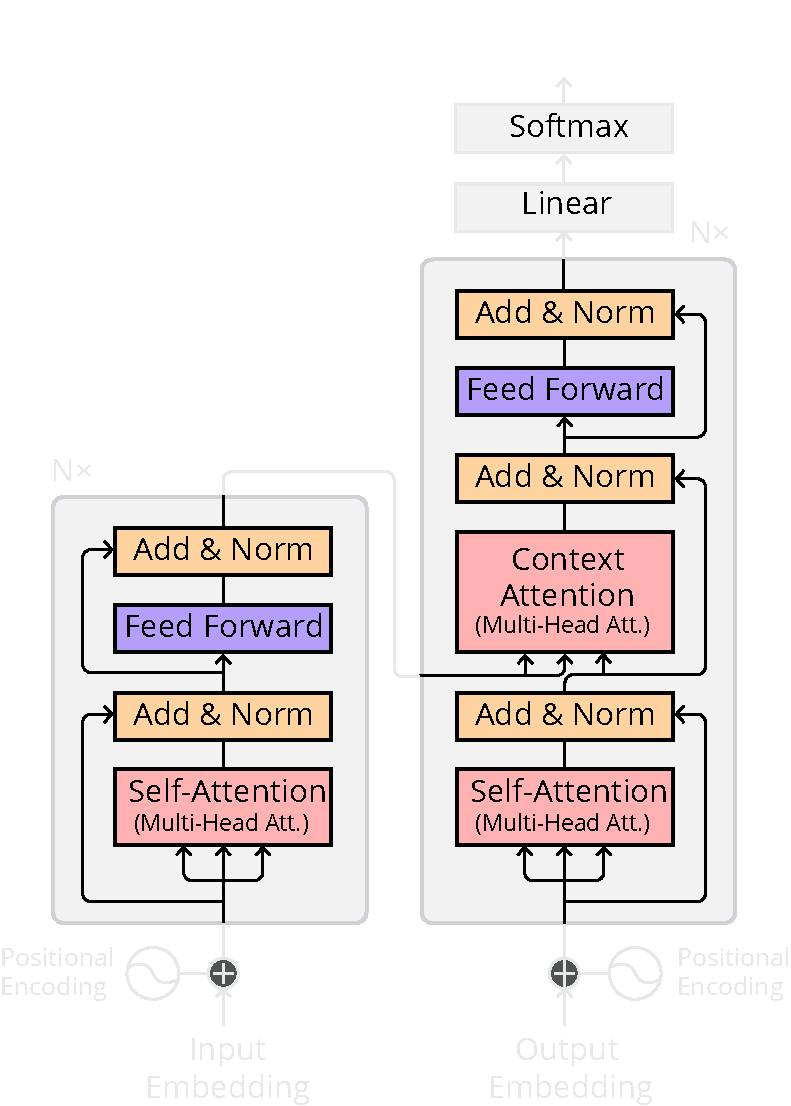
\includegraphics[width=0.9\columnwidth]{figures/transformer_mybg}
%     \tikz[baseline,remember picture]{\node[anchor=base] (t1){};}
%     \end{center}
%     \end{column}
%     \end{columns}

%     \begin{tikzpicture}[remember picture,overlay]   %% use here too
%         \uncover<2>{\path[draw=magenta,ultra thick,->](
%             [xshift=2mm,yshift=1mm]n1.north) to [out=6cm,in=0,distance=-1.5cm] ([xshift=-5.13cm,yshift=2.0cm]t1.north);}
%         \uncover<3>{\path[draw=magenta,ultra thick,->](
%             [xshift=2mm,yshift=1mm]n2.north) to [out=6cm,in=0,distance=-3cm] ([xshift=-2.67cm,yshift=2.0cm]t1.north);}
%         \uncover<4>{\path[draw=magenta,ultra thick,->](
%             [xshift=2mm,yshift=1mm]n3.north) to [out=-6cm,in=0,distance=-2.5cm] ([xshift=-2.67cm,yshift=3.55cm]t1.north);}
%     \end{tikzpicture}
% }

% \begin{itemize}
% \item[]\uncover<6->{
%     {\color{colorEntmax} Key idea:} replace softmax in attention heads by a sparse normalizing function! \quad\emoji{palms}
% }

% \bigskip

% \item[]\uncover<7->{
%     {\color{myDarkYellow} Another key idea:}
%     use a normalizing function that is adaptively sparse via a learnable $\alpha$! \quad\emoji{palms}\enspace\emoji{palms}\enspace\emoji{palms}
% }
% \end{itemize}

% % \bigskip

% % \begin{itemize}
% % \uncover<4->{\item Recall: $\alpha$ controls propensity to sparsity}
% % \uncover<5->{\item Learn each $\alpha \in [1,2]$ {\bf adaptively}!}
% % \uncover<6->{\item One $\alpha$ for each attention head and each layer}
% % \uncover<7->{\item Heads can be dense or sparse, depending on their roles.}
% % \end{itemize}

% \end{frame}

% \begin{frame}[fragile]
%     \frametitle{Related Work: Other Sparse Transformers}
%     \cornercite{Child2019,Sukhbaatar2019}

%     \vspace{-1.5cm}
%     \begin{center}
%     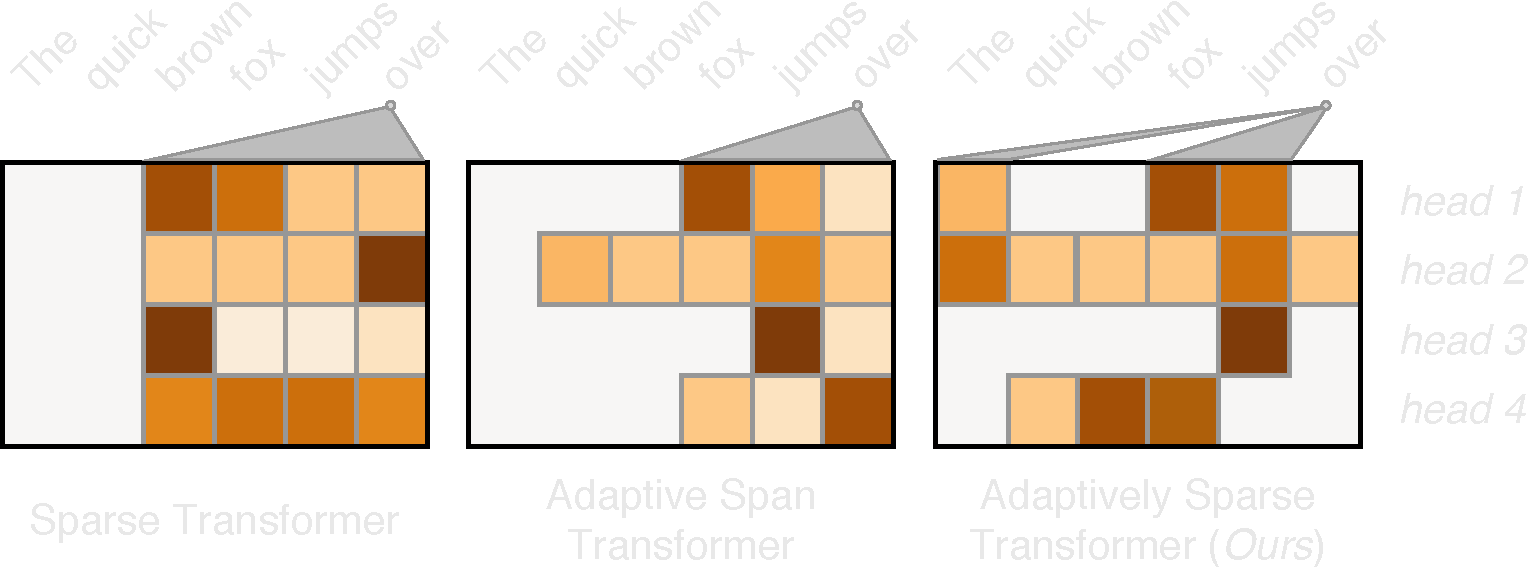
\includegraphics[width=0.7\columnwidth]{figures/comparison_mybg}

%     \bigskip

%     Our model allows {\color{myDarkYellow} non-contiguous} attention for each head.
%     \end{center}

% \end{frame}

% \section{Sparse Transformations}

% \begin{frame}[plain,t,fragile]%
%     \frametitle{What is softmax?}%
%     \centering \fontsize{12pt}{15}\selectfont
%     Softmax exponentiates and normalizes:\quad
%     $\displaystyle
%     \softmax(\xx_i) \defeq \frac{\exp \left(\xx_i\right)}{\sum_j \exp \left(\xx_j\right)}$

%     \uncover<2->{
%     {\color{myDarkYellow} It's fully dense: $\softmax(\vectsymb{z}) > \vect{0}$}}

%     \vspace{1cm}

%     \uncover<3->{Argmax can be written as:\\
%     \vspace{0.5cm}
%     $\displaystyle
%     \argmaxbf(\vectsymb{z}) \defeq \arg\max_{\vectsymb{p} \in \triangle} \DP{\vectsymb{z}}{\vectsymb{p}}$

%     \bigskip

%     \begin{itemize}
%     \item<4-> Retrieves a {\bf one-hot vector} for the highest scored index.
%     \item<5-> Sometimes used as hard attention, but not differentiable!
%     \end{itemize}
%     }
% \end{frame}

% \begin{frame}{$\Omega$-Regularized Argmax}
%     \cornercite{Niculae2017}
%     \fontsize{12pt}{15}\selectfont
%     \vspace{-0.5cm}
%     \begin{itemize}
%     \item[] For convex $\Omega$, define the {\bf $\Omega$-regularized argmax transformation}:\\
%     \bigskip
%     \begin{center}
%     $\displaystyle
%     \argmaxbf{}_{{\Omega}}(\vectsymb{z}) \defeq \arg\max_{\vectsymb{p} \in \triangle} \DP{\vectsymb{z}}{\vectsymb{p}} {\color{tPeony}- \Omega(\vectsymb{p})}$
%     \end{center}
%     \end{itemize}
%     \bigskip
%     \begin{itemize}
%     \uncover<2->{\item {\color{myDarkYellow} Argmax} corresponds to {\bf no regularization}, $\displaystyle\Omega \equiv 0$}
%     \uncover<3->{\item {\color{myDarkYellow} Softmax} amounts to {\bf entropic regularization}, $\displaystyle\Omega(\vectsymb{p}) = \sum_{i=1}^K p_i \log p_i$}
%     \uncover<4->{\item {\color{myDarkYellow} Sparsemax} amounts to {\bf $\ell_2$-regularization}, $\displaystyle\Omega(\vectsymb{p}) = \frac{1}{2}\|\vectsymb{p}\|^2$.}
%     \end{itemize}
%     \bigskip
%     \begin{itemize}
%     \item[] \uncover<5->{Is there something in-between?}
%     \end{itemize}
%     \uncover<4>{\cornercite[south east]{sparsemax}}
% \end{frame}

% \begin{frame}{$\alpha$-Entmax}
%     \cornercite{Peters2019ACL}
%     \vspace{-1cm}
%     \fontsize{12pt}{15}\selectfont
%     \begin{itemize}
%     \item[] Parametrized by {\color{tPeony}$\alpha \ge 0$}:
%     \end{itemize}
%     \bigskip
%     \begin{center}
%     $\displaystyle
%     \Omega_{{\color{tPeony}\alpha}}(\vectsymb{p}) \defeq 
%     \left\{
%     \begin{array}{ll}
%     \frac{1}{\alpha(\alpha-1)} \left(1 - \sum_{i=1}^K p_i^{\alpha}\right) & \text{if $\alpha \ne 1$}\\
%     \sum_{i=1}^K p_i\log p_i & \text{if $\alpha = 1$.}
%     \end{array}
%     \right.$
%     \end{center}
%     \bigskip
%     \begin{itemize}
%         \uncover<2->{\item {\bf Argmax} corresponds to {\color{tPeony}$\alpha \rightarrow \infty$}}
%         \uncover<3->{\item {\bf Softmax} amounts to {\color{tPeony}$\alpha \rightarrow 1$}}
%         \uncover<4->{\item {\bf Sparsemax} amounts to {\color{tPeony}$\alpha = 2$}.}
%     \end{itemize}
%     \bigskip
%     \begin{itemize}
%         \uncover<5->{\item[] {\color{myDarkYellow} Key result:} {\bf can be sparse for $\alpha > 1$}, propensity for sparsity increases with $\alpha$.}
%     \end{itemize}

% \end{frame}

% \section{Efficient Marginalization of Discrete and Structured Latent Variables via Sparsity}

% \begin{frame}
%     \frametitle{Learning $\alpha$}

%     \begin{itemize}
%         \uncover<2->{\item[] {\color{myDarkYellow} Key contribution}: \\\bigskip\quad a closed-form expression for $\pfrac{\aentmax(\x)}{\alpha}$ \quad\emoji{oface}}
%     \end{itemize} 

%     \bigskip

%     \begin{itemize}

%         \uncover<3->{\item[] Requires argmin differentiation $\rightarrow$ see paper for details!}

%     \end{itemize}

%     \uncover<4->{\overlaybox[0.5]{\texttt{:pip install entmax}\\Check \href{https://github.com/deep-spin/entmax}{\tt github.com/deep-spin/entmax}}}

% \end{frame}

% \begin{frame}
%     \frametitle{BLEU Scores}

%     \begin{table}[ht]
%         \begin{center}
%         \small
%         \resizebox{0.8\columnwidth}{!}{\begin{tabular}{lrrrr}
%         \toprule
%         activation
%         & \langp{de}{en} & \langp{ja}{en}
%         & \langp{ro}{en} & \only<1>{\langp{en}{de}}\only<2->{{\color{tPeony} \langp{en}{de}}}\\
%         \midrule
%         $\softmaxlight$
%         & 29.79
%         & 21.57
%         & 32.70
%         & 26.02 \\
%         $\aentmax[1.5]$
%         & 29.83
%         & {\color{myDarkYellow} 22.13}
%         & {\color{myDarkYellow} 33.10}
%         & 25.89 \\
%         $\aentmax[\alpha]$
%         & {\color{myDarkYellow} 29.90}
%         & 21.74
%         & 32.89
%         & {\color{myDarkYellow} 26.93} \\
%         \bottomrule
%         \end{tabular}}
%         \end{center}
%     \end{table}

%     \bigskip

%     \begin{itemize}
%         \uncover<3>{\item[] For analysis for other language pairs, see Appendix A.}
%     \end{itemize}

% \end{frame}

% \section{Conclusions}

% \begin{frame}[fragile]
%   \frametitle{Key Takeaways}

%     \centering\fontsize{14pt}{14}\selectfont%
%     Introduce {\color{myDarkYellow} adaptive} sparsity\\
%     for Transformers via $\alpha$-entmax with a {\color{myDarkYellow}gradient learnable $\alpha$}.
%     %
%     %
%     \vfill
%     %
%     %
%     \begin{columns}[T]
%     \small
%     \begin{column}{.33\textwidth}
%     \centering
%     \uncover<2->{
%     \textbf{\emph{adaptive sparsity}}\\[.5\baselineskip]
%     \vspace{0.2cm}
%     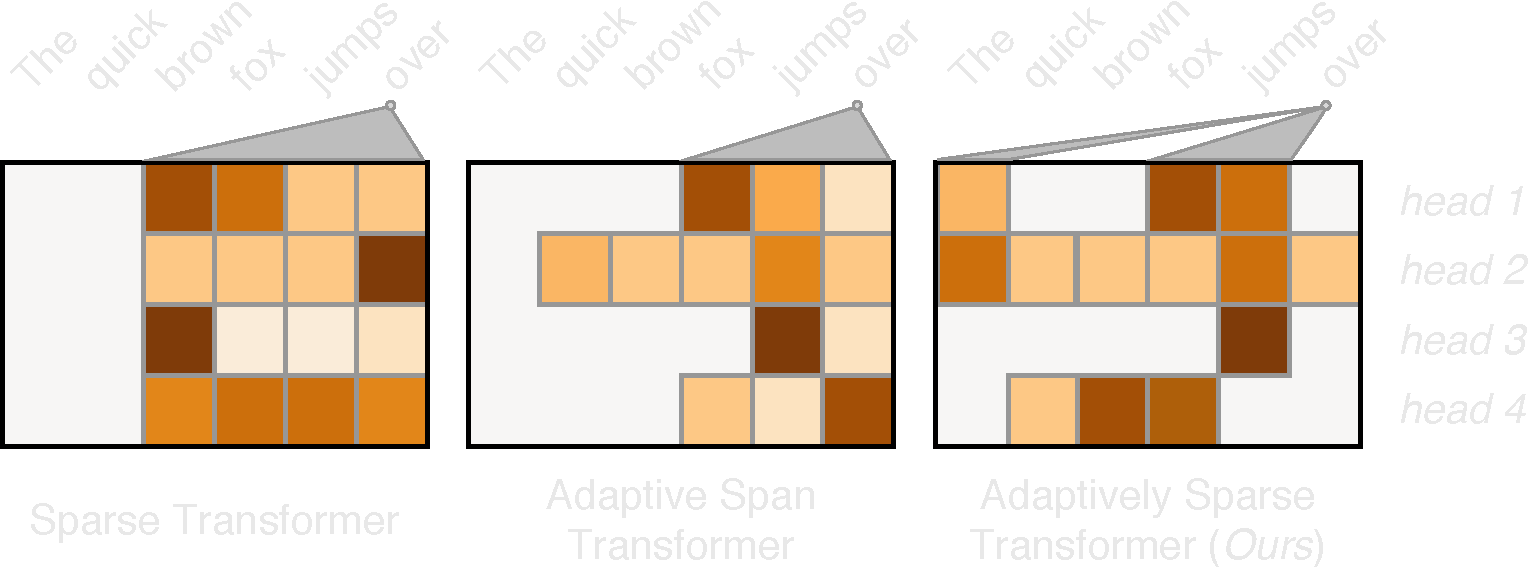
\includegraphics[trim=157mm 17mm 0 0, clip, width=.7\textwidth]{figures/comparison_mybg}}%
%     \end{column}
%     \begin{column}{.33\textwidth}
%     \centering
%     \uncover<3->{
%     \textbf{\emph{reduced head redundancy}}\\[\baselineskip]}
%     \vspace{-0.2cm}
%     \begin{tikzpicture}[node distance=1.5ex,font=\scriptsize,scale=0.5, visible on=<3->]

%         \definecolor{color0}{rgb}{0.12156862745098,0.466666666666667,0.705882352941177}
%         \definecolor{color1}{rgb}{1,0.498039215686275,0.0549019607843137}
%         \definecolor{color2}{rgb}{0.172549019607843,0.627450980392157,0.172549019607843}
        
%         \begin{groupplot}[group style={group size=1 by 1}]
%         \nextgroupplot[
%         legend cell align={left},
%         legend style={
%                 nodes={scale=1.1, transform shape}, at={(0.97,0.2)}, anchor=east, draw=white!80.0!black, fill=myfg!30!mybg},
%         tick align=outside,
%         tick pos=left,
%         x grid style={white!69.01960784313725!black},
%         xmin=0.5, xmax=6.5,
%         xtick = {1, 2, 3, 4, 5, 6},
%         xtick style={color=white},
%         y grid style={white!69.01960784313725!black},
%         ymin=0.1, ymax=0.7,
%         ytick = {0.2, 0.4, 0.6},
%         ytick style={color=white}
%         ]
%         \addplot [thick, color0, mark=square*, mark size=3, mark options={solid}]
%         table {%
%         1 0.38571667343747
%         2 0.402429158203537
%         3 0.440747738282957
%         4 0.359233941813858
%         5 0.337470844946825
%         6 0.339900884621234
%         };
%         \addlegendentry{softmax}
%         \addplot [thick, color1, mark=*, mark size=3, mark options={solid}]
%         table {%
%         1 0.378367748537659
%         2 0.504354104995477
%         3 0.573529792473815
%         4 0.525266398541884
%         5 0.439669581263257
%         6 0.421346772557364
%         };
%         \addlegendentry{1.5-entmax}
%         \addplot [thick, color2, mark=asterisk, mark size=3, mark options={solid}]
%         table {%
%         1 0.427742934860258
%         2 0.484287995253192
%         3 0.533714455762104
%         4 0.449772918584636
%         5 0.3935698561848
%         6 0.355665944457941
%         };
%         \addlegendentry{$\alpha$-entmax}
%     \end{groupplot}
%     \end{tikzpicture}
%     \end{column}
%     \begin{column}{.33\textwidth}
%     \centering
%     \uncover<4->{
%     \textbf{\emph{clearer head roles}}\\[\baselineskip]
%     \vspace{-0.2cm}
%     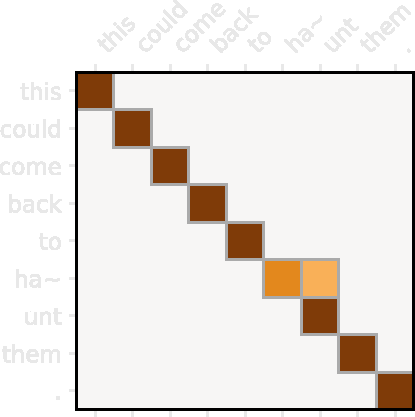
\includegraphics[width=.6\textwidth]{figures/bpe4}}
%     \end{column}
%     \end{columns}

%     \vfill

%     \centering
%     {\scriptsize
%     \color{mygr}
%     \begin{tabular}{r@{~}l@{\quad}r@{~}l}
%     \raisebox{-0.7mm}[\height][\depth]{\emoji{githubfg}}& \href{https://github.com/deep-spin/entmax}{\tt github.com/deep-spin/entmax} &
%     \raisebox{-0.4mm}[\height][\depth]{\emoji{home}}& \href{https://goncalomcorreia.github.io}{\tt goncalomcorreia.github.io}
%     \end{tabular}}

% \end{frame}

% \begin{frame}
%     \centering
%     \vspace{-2cm}
%     \fontsize{30pt}{15}\selectfont
%     Thank you!

%     \bigskip

%     \fontsize{20pt}{15}\selectfont
%     Questions?

%     \overlaybox[0.7]{\texttt{:pip install entmax}\\Check \href{https://github.com/deep-spin/entmax}{\tt github.com/deep-spin/entmax}}
% \end{frame}

% {
% \setbeamercolor{background canvas}{bg=white}
% \setbeamercolor{normal text}{fg=mygr}
% \setbeamercolor{frametitle}{fg=mybg}
% \usebeamercolor[fg]{frametitle}
% \usebeamercolor[fg]{normal text}
% \begin{frame}
% \frametitle{Acknowledgements}
% \centering
% \small
% 
\includegraphics[width=.2\textwidth]{img/erc.png}\\
% This work was supported by the European Research
% Council (ERC StG DeepSPIN 758969) and by the
% Fundação para a Ciência e Tecnologia through contract UID/EEA/50008/2019 and
% CMUPERI/TIC/0046/2014 (GoLocal).
% \end{frame}
% }

\begin{frame}[t,allowframebreaks]
\frametitle{References}
\printbibliography
\end{frame}

\end{document}

